%% ====================================================================
%%  A Concept Guide to the DLoc Compression Thesis
%%  Companion teaching document — E-JUST B.Sc. graduation project
%%
%%  Compile:  pdflatex main  ->  pdflatex main   (twice for TOC/refs)
%%  (or:  latexmk -pdf main.tex).  No bibliography engine needed; the
%%  guide cites the thesis itself rather than maintaining its own .bib.
%%
%%  Each part lives in its own file under chapters/ so the three authors
%%  can study/own different parts independently.
%% ====================================================================
\documentclass[12pt,a4paper,oneside]{report}

%% ====================================================================
%%  preamble.tex — packages, paths, and custom commands for the
%%  DLoc Thesis Concept Guide. Style mirrors thesis/preamble.tex so the
%%  two documents look like a matched set.
%% ====================================================================

\usepackage[utf8]{inputenc}
\usepackage[T1]{fontenc}
\usepackage[english]{babel}

\usepackage{geometry}
\geometry{a4paper, margin=2.5cm}

\usepackage{graphicx}
%% Look in our own figures/ first, then fall back to the thesis/repo figures
%% so the guide compiles in-repo even before figures are copied locally.
\graphicspath{{figures/}{../thesis/figures/}{../Figures/generated/}{../Figures/}}

\usepackage{amsmath,amssymb}
\usepackage{booktabs}
\usepackage{multirow}
\usepackage{array}
\usepackage{tabularx}
\usepackage{float}
\usepackage{caption}
\usepackage{subcaption}
\usepackage[chapter]{placeins}
\usepackage{enumitem}
\usepackage{xcolor}
\usepackage{colortbl}
\usepackage{setspace}
\onehalfspacing
\raggedbottom

%% --- compact chapter titles (match the thesis look) ---
\usepackage{titlesec}
\titleformat{\chapter}[block]
  {\normalfont\bfseries\Huge}{\thechapter\quad}{0pt}{\Huge}
\titlespacing*{\chapter}{0pt}{6pt}{14pt}

\usepackage{tikz}
\usetikzlibrary{positioning, arrows.meta, calc, fit, backgrounds,
  shapes.geometric, shapes.misc, decorations.pathreplacing}

%% --- pedagogical callout boxes (Overleaf / TeX Live full ship tcolorbox) ---
\usepackage[most]{tcolorbox}

\usepackage[hidelinks]{hyperref}
\hypersetup{
  colorlinks=true,
  linkcolor=black,
  citecolor=black,
  urlcolor=blue,
}

%% --- colours + helpers reused from the thesis/results report ---
\definecolor{bestcolor}{RGB}{0,128,0}
\definecolor{worstcolor}{RGB}{180,0,0}
\definecolor{lightgray}{gray}{0.92}
\definecolor{accent}{RGB}{38,70,83}
\definecolor{accent2}{RGB}{42,157,143}
\definecolor{accent3}{RGB}{231,111,81}
\newcommand{\best}[1]{\textcolor{bestcolor}{\textbf{#1}}}
\newcommand{\worst}[1]{\textcolor{worstcolor}{#1}}

%% --- shorthand for the recurring quantities ---
\newcommand{\m}{\,\text{m}}                     % metres
\newcommand{\code}[1]{\texttt{#1}}

%% --- title-page name (matches the thesis); defined before use on the title page ---
\newcommand{\supervisorname}{Prof.\ Ehab Elshazly}

%% --- three callout environments used throughout the guide ---
\newtcolorbox{keyidea}{
  enhanced, breakable, colback=accent2!7, colframe=accent2!75!black,
  boxrule=0.7pt, arc=2pt, left=6pt, right=6pt, top=4pt, bottom=4pt,
  fonttitle=\bfseries, title=Key idea}

\newtcolorbox{whybox}{
  enhanced, breakable, colback=accent!6, colframe=accent!80!black,
  boxrule=0.7pt, arc=2pt, left=6pt, right=6pt, top=4pt, bottom=4pt,
  fonttitle=\bfseries, title=Why it behaved this way}

\newtcolorbox{defensetip}{
  enhanced, breakable, colback=accent3!8, colframe=accent3!80!black,
  boxrule=0.7pt, arc=2pt, left=6pt, right=6pt, top=4pt, bottom=4pt,
  fonttitle=\bfseries, title=Defense tip}

%% --- a compact key/value "at a glance" box for the model deep-dives ---
\newtcolorbox{ataglance}[1]{
  enhanced, breakable, colback=lightgray, colframe=black!55,
  boxrule=0.6pt, arc=1pt, left=6pt, right=6pt, top=3pt, bottom=3pt,
  fonttitle=\bfseries, title=At a glance: #1}


\begin{document}

%% ---------------- Title page ----------------
\begin{titlepage}
\centering
\vspace*{2.2cm}
{\scshape\large A Companion Concept Guide to the Thesis\par}
\vspace{0.4cm}
{\color{accent}\rule{\linewidth}{1.2pt}}\par
\vspace{0.8cm}
{\huge\bfseries Lightweight Knowledge-Distilled\\[0.2em]
Deep Learning for WiFi Indoor Localization\par}
\vspace{0.6cm}
{\Large A Detailed, Concepts-First Study \& Defense Guide\par}
\vspace{0.3cm}
{\color{accent}\rule{\linewidth}{1.2pt}}\par
\vspace{1.4cm}

{\large
This guide teaches every concept the thesis rests on --- from WiFi channel
state information to cumulative error distributions --- dissects each model
architecture and \emph{why} it behaved the way it did, and closes with a
defense question-and-answer bank.\par}
\vspace{2.0cm}

{\large\bfseries Authors\par}
\vspace{0.2cm}
{\large Abdulrahman Mahmoud Ali Ebrahim \\
Ahmed Emadeldin Abdelsallam Haggag \\
Fadwa Yasser Khalil Mahmoud \par}
\vspace{1.0cm}
{\large\textbf{Supervisor:} \supervisorname\ \par}
\vspace{0.2cm}
{\large Egypt--Japan University of Science and Technology (E-JUST)\par}
\vfill
{\large \today\par}
\end{titlepage}

\pagenumbering{roman}
%% ====================================================================
%%  How to Use This Guide  (unnumbered preface)
%% ====================================================================
\chapter*{How to Use This Guide}
\addcontentsline{toc}{chapter}{How to Use This Guide}
\markboth{How to Use This Guide}{}

This document is a \emph{concept-first companion} to the thesis \emph{``Lightweight
Knowledge-Distilled Deep Learning for WiFi Indoor Localization.''} The thesis reports \emph{what} we
did and \emph{what} we found; this guide explains \emph{why} every concept works and \emph{why} every
model behaved the way it did, starting from the foundations. It is written so that each of the three
authors can read any part independently and walk into the defense able to explain --- not just recite
--- the work. It complements the four system-reference documents in \code{docs/}
(\code{01\_dloc\_architecture}, \code{02\_dataset}, \code{03\_model\_architectures},
\code{04\_experiments}); where those say ``here is exactly what our system is,'' this guide teaches
the underlying ideas.

\section*{The thesis in one page}

\textbf{The problem.} GPS does not work indoors, but WiFi access points (APs) are everywhere and
already measure \emph{Channel State Information} (CSI). DLoc~--- a 2020 system from UC San Diego ---
turns CSI into an image and learns to ``translate'' it into a heatmap whose bright spot is the
person's location, reaching sub-meter accuracy. The catch: DLoc has \textbf{16.5 million parameters},
far too heavy for the edge devices (gateways, phones, the APs themselves) where indoor localization
is actually useful.

\textbf{The question.} Is that 16.5\,M cost \emph{inherent} to the task, or is DLoc simply
over-parameterized? If it is over-parameterized, how small a model can still localize accurately, and
what do we lose along the way?

\textbf{What we did.} We compressed DLoc into a family of lightweight ``student'' models
---MobileNetV2 (2.3\,M), a minimal TinyCNN (47\,K), a MobileNetV2 encoder with U-Net skip connections
(2.41\,M), and a state-space Mamba model (0.65\,M)--- and trained each one both \emph{standalone} and
\emph{distilled} from the DLoc teacher. We then evaluated all of them along five axes: in-distribution
accuracy, robustness to signal degradation, cross-session generalization, statistical reproducibility,
and computational efficiency.

\textbf{The headline result.} A \textbf{MobileNetV2-UNet with only 2.41\,M parameters reaches
0.640\,m median error}---\emph{better} than the 0.707\,m DLoc baseline---while using $6.8\times$ fewer
parameters and $56\times$ fewer floating-point operations. The cost of DLoc is therefore \emph{not}
inherent: a model an order of magnitude smaller can match or beat it.

\begin{keyidea}
The thesis is fundamentally an \textbf{efficiency} result wrapped around a \textbf{scientific} one.
The efficiency result: an order-of-magnitude-smaller model matches DLoc. The scientific result: the
two ways we made the small model good---\emph{U-Net skip connections} and \emph{knowledge
distillation}---improve different kinds of \emph{robustness}, and distillation only helps models above
a capacity threshold of about 2\,M parameters.
\end{keyidea}

\section*{The argument, as a chain}

Read the thesis as a single chain of claims; every chapter of this guide deepens one link:

\begin{enumerate}[leftmargin=2.2em]
  \item Localization can be framed as \emph{image-to-image translation} from CSI heatmaps to a
  location heatmap (Ch.~\ref{ch:foundations}).
  \item The building blocks that make a network small \emph{and} good are convolutions, skip
  connections, depthwise-separable convolutions, and U-Net skips (Ch.~\ref{ch:blocks}).
  \item \emph{Knowledge distillation} can transfer a big teacher's behavior into a small student
  (Ch.~\ref{ch:distill}); for our heatmap task it acts as ``spatial label smoothing.''
  \item We measure everything with a pixel-distance error and its \emph{distribution} ---median, P90,
  P99, mean, and the CDF (Ch.~\ref{ch:eval}).
  \item Each architecture then behaves in a specific, explainable way ---the over-parameterized
  teacher, the lossless MobileNetV2, the under-capacity TinyCNN, the teacher-beating U-Net, the
  mismatched Mamba (Ch.~\ref{ch:arch}).
  \item Comparing them yields six findings about compression, architecture, and distillation
  (Ch.~\ref{ch:findings}).
  \item Finally, anticipate the committee's questions (Ch.~\ref{ch:qa}).
\end{enumerate}

\section*{How to read it, depending on your goal}

\begin{itemize}[leftmargin=1.4em]
  \item \textbf{``I want to understand the whole thing.''} Read front to back. Each chapter assumes
  the previous one.
  \item \textbf{``I own the architecture questions.''} Read Ch.~\ref{ch:blocks} (concepts) then
  Ch.~\ref{ch:arch} (each model).
  \item \textbf{``I own distillation/robustness.''} Read Ch.~\ref{ch:distill} and Ch.~\ref{ch:eval},
  then findings 3--5 in Ch.~\ref{ch:findings}.
  \item \textbf{``I want to rehearse.''} Go straight to the Defense Q\&A (Ch.~\ref{ch:qa}) and the
  cheat-sheet in Appendix~\ref{app:glossary}; follow each answer's cross-reference back when a concept
  is shaky.
\end{itemize}

\section*{Concept-to-thesis map}

Table~\ref{tab:concept_map} points each concept to where it lives in the thesis, so this guide and the
thesis stay in lock-step.

\begin{table}[H]
\centering
\caption{Where each concept appears in the thesis.}
\label{tab:concept_map}
\small
\begin{tabular}{@{}lll@{}}
\toprule
\textbf{Concept} & \textbf{This guide} & \textbf{Thesis location} \\
\midrule
CSI, AoA/ToF, image-translation framing & Ch.~\ref{ch:foundations} & Sec.~3.1, docs/01--02 \\
Conv / encoder--decoder / skips         & Ch.~\ref{ch:blocks}      & Sec.~2.3 \\
Depthwise-separable, inverted residuals & Ch.~\ref{ch:blocks}      & Sec.~2.3.2 \\
U-Net skip connections                  & Ch.~\ref{ch:blocks}      & Sec.~2.3.3, 3.3.3 \\
State-space models / Mamba              & Ch.~\ref{ch:blocks}      & Sec.~2.3.4, 3.3.4 \\
Knowledge distillation                  & Ch.~\ref{ch:distill}     & Sec.~2.2, 3.4 \\
Error metric, percentiles, CDF          & Ch.~\ref{ch:eval}        & Sec.~3.6, 5.1 \\
Robustness corruptions                  & Ch.~\ref{ch:eval}        & Sec.~3.5, 4.4, 5.3 \\
Cross-session (LOSO / zero-shot)        & Ch.~\ref{ch:eval}        & Sec.~4.5, 5.4 \\
Per-model results \& reasons            & Ch.~\ref{ch:arch}        & Ch.~5 (all) \\
The six findings                        & Ch.~\ref{ch:findings}    & Ch.~5--6 \\
\bottomrule
\end{tabular}
\end{table}

A running convention: green bold marks a \best{best} result and red marks a \worst{worst} result, the
same as in the thesis tables.


\tableofcontents
\listoffigures
\clearpage

%% ---------------- Body ----------------
\pagenumbering{arabic}
%% ====================================================================
%%  Chapter 1 — Foundations: WiFi Localization and the CSI Signal
%% ====================================================================
\chapter{Foundations: WiFi Localization and the CSI Signal}
\label{ch:foundations}

Before any neural network appears, you need to understand the physical problem and the clever
reframing that makes deep learning applicable to it. This chapter builds that foundation: why indoor
localization is hard, what a WiFi signal actually measures, how that measurement becomes an
``image,'' and why the whole problem is then solved as \emph{image-to-image translation}.

\section{Why indoor localization, and why GPS fails indoors}
\label{sec:found:gps}

Many applications need to know \emph{where} something is inside a building: tracking assets in a
warehouse, finding patients in a hospital, augmented reality, indoor robots, and location-aware
services in malls or airports. Outdoors, GPS solves this to within a few meters. Indoors, it
collapses.

GPS works by timing signals from satellites in direct line of sight. Indoors, those signals are
\emph{attenuated} (weakened) by walls and roofs and \emph{reflected} off surfaces, so a receiver sees
a jumble of delayed copies rather than a clean direct path. The timing that GPS depends on is
destroyed. Two decades of research therefore looked for indoor alternatives: WiFi, Bluetooth,
ultra-wideband, and inertial sensors.

\begin{keyidea}
The same physics that breaks GPS indoors ---reflection and \emph{multipath}--- is exactly what an
indoor WiFi system must learn to cope with. Our models do not avoid multipath; they learn to read
through it.
\end{keyidea}

\section{The WiFi opportunity: access points and CSI}
\label{sec:found:wifi}

WiFi is the most studied indoor-localization technology for one practical reason: the infrastructure
already exists. Almost every building is blanketed by WiFi access points (APs). And modern WiFi
hardware, as a side effect of doing its real job (reliable communication), continuously measures
something extremely useful for localization: \textbf{Channel State Information (CSI)}.

When an AP communicates with a device, it must estimate how the wireless channel distorted the
signal so it can undo that distortion. That per-channel estimate \emph{is} the CSI. Because the way a
signal is distorted depends on the geometry between the device and the AP ---distance, angle, what it
bounced off--- the CSI implicitly encodes \emph{where the device is}. Extracting that location is the
whole game.

\section{What CSI physically is}
\label{sec:found:csi}

WiFi uses \emph{orthogonal frequency-division multiplexing} (OFDM): instead of one carrier frequency,
the signal is split across many narrow \textbf{subcarriers}. For each subcarrier (and each antenna on
the AP), the hardware estimates a single complex number describing how that frequency was attenuated
and phase-shifted by the channel. Stack those numbers up and you get the CSI matrix at AP~$i$:
\[
  H_i \in \mathbb{C}^{\,N_{\text{sub}} \times N_{\text{ant}}},
\]
with $N_{\text{sub}}$ subcarriers and $N_{\text{ant}}$ antennas. Each entry has an \emph{amplitude}
(how much the signal weakened) and a \emph{phase} (how much it was delayed, modulo a wavelength).

Two facts make CSI informative about location:
\begin{itemize}[leftmargin=1.4em,nosep]
  \item \textbf{Amplitude vs.\ distance.} Signal strength falls off with distance, so amplitude is a
  (noisy) distance cue.
  \item \textbf{Phase across antennas vs.\ angle.} A wavefront arriving at an angle hits the AP's
  antennas at slightly different times, producing a predictable phase progression across the antenna
  array. That progression encodes the \emph{angle of arrival}.
\end{itemize}

\section{From CSI to a per-AP heatmap: AoA and ToF}
\label{sec:found:aoa}

Raw complex CSI is not something you would feed a vision network directly. DLoc's pre-processing
(done in MATLAB, ``stage 0'' of the pipeline) turns each AP's CSI into a 2D \textbf{Angle-of-Arrival
/ Time-of-Flight (AoA--ToF) profile} and then projects it onto the physical floor grid. The result is
a per-AP \emph{heatmap} over the room: bright where ``the signal looks like it came from here.''

\begin{itemize}[leftmargin=1.4em,nosep]
  \item \textbf{Angle of Arrival (AoA)} ---from the phase progression across antennas--- says
  \emph{which direction} the signal came from.
  \item \textbf{Time of Flight (ToF)} ---from the phase progression across subcarriers (frequencies)---
  says \emph{how far} the signal travelled.
\end{itemize}

Combine direction and distance for one AP and you get a constraint on where the device is; combine
the constraints from several APs and you can, in principle, pin down the location. For the Jacobs
Hall environment used throughout the thesis there are $N_{\text{AP}}=4$ APs, and each heatmap is
sampled on a $161 \times 361$ grid at $0.1$\,m per pixel ---i.e.\ a $16.1 \times 36.1$\,m floor.
Stacking the four per-AP heatmaps gives a four-channel ``image'' of shape $[\,4,\,161,\,361\,]$.

\begin{figure}[H]
\centering
\begin{tikzpicture}[
  font=\small,
  stage/.style={draw=accent,fill=accent!8,rounded corners,minimum height=1.05cm,
    minimum width=2.5cm,align=center},
  arr/.style={-{Stealth[length=2.4mm]},accent,thick}]
\node[stage] (csi) {Raw CSI\\$H_i\in\mathbb{C}^{N_\text{sub}\times N_\text{ant}}$\\(4 APs)};
\node[stage,right=0.9cm of csi] (prof) {AoA--ToF\\profiles\\(MATLAB)};
\node[stage,right=0.9cm of prof] (img) {4-channel\\input image\\$[4,161,361]$};
\node[stage,right=0.9cm of img,fill=accent2!12,draw=accent2!70!black] (net) {Neural\\network\\(translate)};
\node[stage,right=0.9cm of net] (out) {Output\\heatmap\\$[1,161,361]$};
\node[stage,below=0.7cm of out] (xy) {$\arg\max$\\$\Rightarrow (x,y)$};
\draw[arr] (csi) -- (prof);
\draw[arr] (prof) -- (img);
\draw[arr] (img) -- (net);
\draw[arr] (net) -- (out);
\draw[arr] (out) -- (xy);
\end{tikzpicture}
\caption{The end-to-end pipeline. Physics and signal processing turn raw CSI into a four-channel
``image'' (one channel per AP); the neural network translates that into a single-channel location
heatmap; the brightest pixel, scaled by $0.1$\,m/pixel, is the predicted position.}
\label{fig:found:pipeline}
\end{figure}

\section{The clock-offset problem}
\label{sec:found:offset}

There is a crucial wrinkle. ToF is a \emph{timing} measurement, and the device's clock is not
synchronized with the AP's clock. An unknown clock offset adds an unknown delay to every ToF, which
shifts each AP's heatmap \emph{radially} ---the apparent location can move by $10$--$15$\,m. Worse,
each AP has its own offset, so the four per-AP heatmaps do \emph{not} agree on a single point. The
preprocessing therefore produces two versions of the per-AP heatmaps:
\begin{itemize}[leftmargin=1.4em,nosep]
  \item \code{features\_w\_offset}: \emph{with} the offset present ---this is the network input
  (it is all you would have at deployment);
  \item \code{features\_wo\_offset}: with the offset removed using extra information available only at
  training time ---this is a \emph{training target} that teaches the network to undo the offset.
\end{itemize}
This is the single most important reason a \emph{learned} system beats classical geometry here:
resolving the offset and reconciling four disagreeing APs is exactly what the network learns to do
(the DLoc ``consistency decoder''; see Ch.~\ref{ch:arch} and \code{docs/01}).

\section{Localization as image-to-image translation}
\label{sec:found:translation}

Now the reframing that makes everything click. Instead of computing the location with geometry, DLoc
treats the four-channel CSI image as the \emph{input} of an \textbf{image-to-image translation}
problem ---the same family of problems as ``turn this sketch into a photo''--- and learns a network
that outputs a clean, single-channel heatmap. The target heatmap is a 2D \emph{Gaussian bump}
centered on the true location (\code{labels\_gaussian\_2d}, shape $[1,161,361]$). At test time the
prediction is read off as the \textbf{argmax} of the output heatmap, scaled by $0.1$\,m/pixel; the
error is the Euclidean distance from that pixel to the true one (formalized in Ch.~\ref{ch:eval}).

\begin{keyidea}
Three reframings turn a hard physics problem into a tractable learning problem: (1) represent each
AP's signal as a \emph{spatial heatmap} over the floor; (2) make the network's job \emph{translate
input heatmaps into one output heatmap}; (3) read the location off as the \emph{peak}. Every model in
this thesis ---except Mamba--- accepts this image framing, which is precisely why Mamba struggles
(Ch.~\ref{ch:arch}).
\end{keyidea}

\section{Why deep learning instead of classical geometry}
\label{sec:found:why_dl}

Classical methods (e.g.\ SpotFi) estimate AoA and ToF analytically and intersect them. They work in
clean, line-of-sight conditions but degrade badly under \emph{non-line-of-sight} (NLOS) and rich
indoor multipath, where the strongest path is often a reflection, not the direct one. A learned
network can instead exploit statistical regularities across the four APs and across the training
environment: it can pick the direct path by cross-checking APs, sharpen blurry profiles, and undo
the clock offset. The price for this capability is model size ---and shrinking that price, without
losing the capability, is the subject of the rest of this guide.

%% ====================================================================
%%  Chapter 2 — Architecture Concepts: the Deep-Learning Building Blocks
%% ====================================================================
\chapter{Architecture Concepts: the Building Blocks}
\label{ch:blocks}

Every model in the thesis is assembled from a small set of reusable ideas. This chapter teaches each
idea \emph{once}, generically, so that Chapter~\ref{ch:arch} can simply say ``this model uses
depthwise-separable convolutions and U-Net skips'' and you will already know what that means and why
it matters. For each block we note which thesis model relies on it.

\section{Convolutions: locality and weight sharing}
\label{sec:blocks:conv}

A convolutional layer slides a small learnable filter (say $3\times3$) across the image and computes a
weighted sum at every position. Two properties make this ideal for our heatmaps:
\begin{itemize}[leftmargin=1.4em,nosep]
  \item \textbf{Locality.} Each output pixel depends only on a small neighborhood of the input, which
  matches the fact that a bright spot in a CSI heatmap is a \emph{local} feature.
  \item \textbf{Weight sharing.} The \emph{same} filter is reused at every position, so the layer has
  few parameters and detects a feature wherever it appears. A network needs far fewer weights than a
  fully connected layer would.
\end{itemize}
A convolution layer with a $D_k\times D_k$ kernel, $M$ input channels and $N$ output channels, applied
to a $D_F\times D_F$ feature map, costs
\[
  \underbrace{D_k \cdot D_k \cdot M \cdot N \cdot D_F \cdot D_F}_{\text{multiply--accumulate operations}}
\]
operations. Keep this formula in mind ---the MobileNet trick (Sec.~\ref{sec:blocks:dwsep}) attacks the
$M\cdot N$ factor in it.

\begin{keyidea}
Convolutions are cheap and spatially aware, which is why every \emph{successful} model here is
convolutional. The one model that abandons convolution for a 1D sequence view ---Mamba--- is the one
that fails.
\end{keyidea}

\section{Encoder--decoder networks and the bottleneck}
\label{sec:blocks:encdec}

Image-to-image translation networks have a characteristic hourglass shape:
\begin{itemize}[leftmargin=1.4em,nosep]
  \item an \textbf{encoder} repeatedly \emph{downsamples} (via stride-2 convolutions or pooling),
  shrinking spatial size while growing the number of channels, until the image is compressed into a
  small, deep \textbf{bottleneck} (latent) representation;
  \item a \textbf{decoder} then \emph{upsamples} (via transposed convolutions) back to the original
  resolution to produce the output heatmap.
\end{itemize}
The encoder discovers \emph{what} is in the image; the decoder decides \emph{where} to place the
output. DLoc, MobileNetV2, and the U-Net all share this skeleton. The catch is the bottleneck: by the
time the image has been squeezed to the latent, fine spatial detail has been thrown away ---and for a
\emph{localization} task, spatial detail is precisely the answer. This tension is what skip
connections (next two sections) exist to resolve.

\section{Residual (skip) connections}
\label{sec:blocks:resnet}

Very deep stacks of layers are hard to train: gradients shrink as they propagate backward and the
network struggles to even learn the identity function. \textbf{ResNet} solved this with a
\emph{residual} (or \emph{skip}) connection: instead of asking a block to compute a target mapping
$\mathcal{H}(x)$ directly, you let it compute a residual $\mathcal{F}(x)$ and add the input back,
\[
  y = \mathcal{F}(x) + x .
\]
The $+x$ shortcut gives gradients a direct highway backward (enabling very deep networks) and lets a
block ``do nothing'' easily when that is best. DLoc's encoder and decoders are built from residual
blocks. The same shortcut philosophy ---route information \emph{past} intervening layers--- reappears,
in a different form, as the U-Net skips that power our best model.

\section{Depthwise-separable convolutions (the MobileNet trick)}
\label{sec:blocks:dwsep}

This is the single most important efficiency idea in the thesis. A standard convolution mixes
information across \emph{space} and across \emph{channels} at the same time, which is what makes the
$M\cdot N$ term in its cost so large. A \textbf{depthwise-separable} convolution factorizes that one
operation into two cheaper ones:
\begin{enumerate}[leftmargin=1.6em,nosep]
  \item a \textbf{depthwise} convolution ---one $D_k\times D_k$ filter \emph{per input channel},
  mixing only over space, not channels (cost $D_k\,D_k\,M\,D_F\,D_F$);
  \item a \textbf{pointwise} ($1\times1$) convolution ---mixing only over channels, not space (cost
  $M\,N\,D_F\,D_F$).
\end{enumerate}
The combined cost relative to a standard convolution is
\[
  \frac{D_k D_k\,M + M N}{D_k D_k\,M N} \;=\; \frac{1}{N} + \frac{1}{D_k^{2}} .
\]
For the usual $3\times3$ kernels this is roughly $\tfrac19$ ---an \textbf{$8$--$9\times$ reduction} in
multiply--accumulate operations for nearly the same representational power.

\begin{figure}[H]
\centering
\begin{tikzpicture}[font=\small,
  blk/.style={draw,rounded corners,minimum height=0.85cm,minimum width=2.7cm,align=center},
  arr/.style={-{Stealth[length=2.2mm]},thick}]
% standard
\node[blk,fill=accent3!12,draw=accent3!70!black] (std) {Standard $3{\times}3$\\mix space \emph{and} channels};
\node[align=center,below=2pt of std,font=\footnotesize] {cost $\propto D_k^2 M N$};
% separable
\node[blk,fill=accent2!14,draw=accent2!70!black,right=2.6cm of std,yshift=0.65cm] (dw) {Depthwise $3{\times}3$\\(space only, per channel)};
\node[blk,fill=accent2!14,draw=accent2!70!black,below=0.55cm of dw] (pw) {Pointwise $1{\times}1$\\(channels only)};
\node[align=center,below=2pt of pw,font=\footnotesize] {cost $\propto (D_k^2 M + MN)$};
\draw[arr] (dw) -- (pw);
\node[font=\Large] at ($(std)!0.5!(dw)+(0,-0.32)$) {$\Rightarrow$};
\end{tikzpicture}
\caption{A standard convolution (left) mixes spatial \emph{and} channel information in one expensive
step. The depthwise-separable factorization (right) splits it into a cheap spatial mix (depthwise)
followed by a cheap channel mix (pointwise), cutting cost by $\sim$$8$--$9\times$.}
\label{fig:blocks:dwsep}
\end{figure}

\begin{keyidea}
Depthwise-separable convolutions are \emph{why} a 2.3\,M-parameter MobileNetV2 can do the work of
16.5\,M-parameter DLoc. They buy compression almost for free by separating ``where'' (depthwise) from
``what'' (pointwise). Used by: MobileNetV2, MobileNetV2-UNet.
\end{keyidea}

\section{Inverted residuals and linear bottlenecks (MobileNetV2)}
\label{sec:blocks:invres}

MobileNetV2 wraps depthwise-separable convolutions in an \textbf{inverted residual} block. A classic
residual block is \emph{wide $\to$ narrow $\to$ wide} with the skip on the wide tensors. MobileNetV2
inverts this to \emph{narrow $\to$ wide $\to$ narrow}:
\begin{enumerate}[leftmargin=1.6em,nosep]
  \item \textbf{Expand}: a $1\times1$ convolution widens the channels by a factor $t$ (typically~6).
  \item \textbf{Depthwise}: a $3\times3$ depthwise convolution filters in the wide space.
  \item \textbf{Project}: a $1\times1$ convolution compresses back to a narrow output, with
  \emph{no} activation ---a \textbf{linear bottleneck}.
\end{enumerate}
Two subtleties matter. The skip connects the \emph{narrow} bottleneck tensors (so it moves little
data, saving memory ---``inverted''). And the projection is \emph{linear} because applying a ReLU in
a low-dimensional space destroys information (ReLU zeroes out negatives, and there is no room to spare
in a narrow tensor). The result is a block that keeps a small memory footprint while still computing
in a rich, high-dimensional space. Used by: MobileNetV2, MobileNetV2-UNet.

\section{U-Net skip connections}
\label{sec:blocks:unet}

Recall the bottleneck problem (Sec.~\ref{sec:blocks:encdec}): the encoder discards fine spatial detail
that a localization decoder desperately needs. \textbf{U-Net} fixes this directly. As the encoder
downsamples, it \emph{saves} its intermediate feature maps; as the decoder upsamples, it
\emph{concatenates} the matching-resolution encoder feature map onto the decoder's tensor before the
next convolution. High-resolution detail therefore reaches the output through a short path that
\emph{bypasses the bottleneck} entirely.

\begin{figure}[H]
\centering
\begin{tikzpicture}[font=\small,
  enc/.style={draw=accent,fill=accent!10,minimum width=1.4cm,minimum height=0.8cm,align=center},
  dec/.style={draw=accent2!70!black,fill=accent2!14,minimum width=1.4cm,minimum height=0.8cm,align=center},
  bott/.style={draw=accent3!70!black,fill=accent3!16,minimum width=1.4cm,minimum height=0.8cm,align=center},
  arr/.style={-{Stealth[length=2mm]},thick},
  skip/.style={-{Stealth[length=2mm]},accent2!70!black,thick,dashed}]
\node[enc] (e1) {Enc 1};
\node[enc,below right=0.45cm and 0.5cm of e1] (e2) {Enc 2};
\node[bott,below right=0.45cm and 0.5cm of e2] (b) {Bottle-\\neck};
\node[dec,above right=0.45cm and 0.5cm of b] (d2) {Dec 2};
\node[dec,above right=0.45cm and 0.5cm of d2] (d1) {Dec 1};
\draw[arr] (e1) -- (e2); \draw[arr] (e2) -- (b);
\draw[arr] (b) -- (d2); \draw[arr] (d2) -- (d1);
\draw[skip] (e1) to[out=0,in=180] node[above,font=\footnotesize,black]{concat} (d1);
\draw[skip] (e2) to[out=0,in=180] node[above,font=\footnotesize,black]{concat} (d2);
\end{tikzpicture}
\caption{U-Net skips (dashed) concatenate each encoder stage's high-resolution feature map directly
into the decoder at the matching resolution, so spatial detail bypasses the lossy bottleneck. Our
model concatenates encoder/decoder feature maps of $320{+}96$, $128{+}32$, and $64{+}24$ channels at
its three skip levels.}
\label{fig:blocks:unet}
\end{figure}

\begin{keyidea}
U-Net skips are the reason our 2.41\,M model \emph{beats} its 16.5\,M teacher: they restore the
spatial precision the bottleneck throws away. As a bonus (Ch.~\ref{ch:arch}--\ref{ch:findings}), the
shallow features they carry are also less corrupted by noise, giving ``free'' robustness. Used by:
MobileNetV2-UNet.
\end{keyidea}

\section{State-space models and Mamba}
\label{sec:blocks:mamba}

The last building block is the odd one out. \textbf{State-space models} (SSMs) come from sequence
modeling, an alternative to attention/Transformers. An SSM maintains a hidden state $h_t$ that it
rolls forward one step at a time along a sequence:
\[
  h_t = \bar{A}\,h_{t-1} + \bar{B}\,u_t, \qquad y_t = C\,h_t ,
\]
where $u_t$ is the input at step $t$ and $\bar A,\bar B,C$ are (discretized) state matrices.
\textbf{Mamba} makes this \emph{selective}: the matrices $\bar A,\bar B,C$ (and the time step) become
\emph{functions of the input}, so the model can choose what to remember and what to forget based on
content ---all in linear time over the sequence length, via a hardware-efficient parallel scan.

\begin{figure}[H]
\centering
\begin{tikzpicture}[font=\small,
  st/.style={draw=accent,fill=accent!8,circle,minimum size=0.8cm},
  io/.style={font=\footnotesize},
  arr/.style={-{Stealth[length=2mm]},thick}]
\foreach \i in {1,2,3,4} {
  \node[st] (h\i) at (\i*2,0) {$h_{\i}$};
  \node[io,below=0.45cm of h\i] (u\i) {$u_{\i}$};
  \node[io,above=0.45cm of h\i] (y\i) {$y_{\i}$};
  \draw[arr] (u\i) -- (h\i);
  \draw[arr] (h\i) -- (y\i);
}
\foreach \i/\j in {1/2,2/3,3/4} {\draw[arr] (h\i) -- (h\j);}
\node[io,left=0.5cm of h1] {$\dots$};
\node[io,right=0.5cm of h4] {$\dots$};
\end{tikzpicture}
\caption{An SSM unrolled along a sequence: the hidden state $h_t$ carries information forward
\emph{one step at a time} in a fixed 1D order. This is a natural fit for text or audio ---and a poor
fit for a 2D spatial heatmap, which has no canonical 1D ordering.}
\label{fig:blocks:ssm}
\end{figure}

The crucial point for this thesis is the \emph{inductive bias}: an SSM is built around a
\textbf{one-dimensional, ordered} sequence. To apply it to an image you must first \emph{flatten} the
2D grid into a 1D sequence, which imposes an arbitrary scan order and tears apart pixels that are
spatial neighbors but far apart in the flattened order. As Chapter~\ref{ch:arch} shows, this mismatch
---not a lack of capacity--- is exactly why our Mamba variant failed to learn the heatmap task. Used
by: the Mamba student (as a deliberate ``different inductive bias'' experiment).

%% ====================================================================
%%  Chapter 3 — Knowledge Distillation
%% ====================================================================
\chapter{Knowledge Distillation}
\label{ch:distill}

Knowledge distillation (KD) is the second of the two levers the thesis pulls (the first being
architecture). It is the mechanism by which a small ``student'' learns to behave like a large
``teacher.'' This chapter explains the original idea, then the twist that makes it work for a
\emph{heatmap regression} problem instead of classification, and previews \emph{why} ---in our task---
it turns out to help robustness rather than raw accuracy.

\section{The original idea: soft targets and dark knowledge}
\label{sec:distill:hinton}

KD was introduced by Hinton, Vinyals, and Dean. The setup: you already have a big, accurate
\textbf{teacher} network, and you want a small \textbf{student} that runs cheaply but behaves the
same. The student is trained against two targets at once:
\begin{itemize}[leftmargin=1.4em,nosep]
  \item the usual \textbf{hard labels} (the ground truth), and
  \item the teacher's \textbf{soft labels} ---its full output distribution, not just its top answer.
\end{itemize}
In a classifier, the hard label is one-hot (``this is a cat,'' i.e.\ $[0,1,0,\dots]$). The teacher's
soft label, by contrast, might say ``$90\%$ cat, $9\%$ dog, $1\%$ car.'' That extra structure ---the
fact that the teacher thinks cat is much more like dog than like car--- is what Hinton called
\textbf{dark knowledge}: information about how classes relate that the one-hot label simply does not
contain. Soft labels are usually produced by dividing the logits by a \emph{temperature} before the
softmax, which deliberately smooths the distribution to expose this structure.

\section{Why soft targets help}
\label{sec:distill:why}

Soft targets help for two compounding reasons:
\begin{enumerate}[leftmargin=1.6em,nosep]
  \item \textbf{Richer supervision.} Each training example carries a whole distribution of
  information instead of a single bit, so the student learns more per example.
  \item \textbf{Regularization.} The smoothed target discourages the student from becoming
  over-confident and pushes its internal features toward the teacher's better-behaved ones, which
  tends to generalize better.
\end{enumerate}
Hold on to the \emph{regularization} view ---it is the one that carries over to our task.

\section{Distillation for a heatmap regression task}
\label{sec:distill:ours}

Our task is not classification: the target is a \emph{spatial heatmap}, a 2D Gaussian bump over the
floor (Ch.~\ref{ch:foundations}). This changes distillation in a subtle but important way. There is no
softmax and no temperature to tune ---but the teacher's output is \emph{already soft by
construction}. DLoc does not emit a single hard pixel; it emits a heatmap with probability mass
\emph{spread around} the predicted location, reflecting its own uncertainty. That spread is exactly
the analogue of dark knowledge: it encodes ``the device is most likely here, but plausibly in this
surrounding region.''

\begin{keyidea}
In classification, you must \emph{manufacture} soft targets by raising the softmax temperature. In our
heatmap task, the teacher's targets are \emph{born soft}: the Gaussian-like spread of probability mass
around the location is the dark knowledge. Distillation here is therefore a form of \textbf{spatial
label smoothing}.
\end{keyidea}

\section{The combined loss and teacher precomputation}
\label{sec:distill:loss}

Each student is trained in two modes: \textbf{standalone} (ground truth only) and \textbf{distilled}
(ground truth plus teacher). The distilled objective is a convex combination of a ground-truth term
and a teacher-matching term:
\[
  \mathcal{L} \;=\; \alpha\cdot \mathrm{MSE}(\hat{y},\,y) \;+\; \beta\cdot \mathrm{MSE}(\hat{y},\,y_T),
  \qquad \alpha = 0.7,\;\; \beta = 0.3,
\]
where $\hat y$ is the student's predicted heatmap, $y$ is the ground-truth Gaussian, and $y_T$ is the
teacher's output heatmap. The weights $0.7/0.3$ keep the ground truth dominant while letting the
teacher's softer target gently regularize the student.

A practical implementation detail makes this tractable. The teacher is \emph{fixed}, so its output for
every training and test example is \textbf{precomputed once and cached to disk} ($\approx$4.09\,GB for
the training split, $\approx$0.99\,GB for the test split). During student training, $y_T$ is just read
from cache ---the 16.5\,M-parameter teacher is \emph{never} run in the training loop. This is what
makes it feasible to distill many students across many random seeds.

\begin{figure}[H]
\centering
\begin{tikzpicture}[font=\small,
  big/.style={draw=accent,fill=accent!10,rounded corners,minimum width=2.6cm,minimum height=0.95cm,align=center},
  small/.style={draw=accent2!70!black,fill=accent2!14,rounded corners,minimum width=2.6cm,minimum height=0.95cm,align=center},
  data/.style={draw=black!55,fill=lightgray,rounded corners,minimum width=2.2cm,minimum height=0.85cm,align=center},
  arr/.style={-{Stealth[length=2.2mm]},thick},
  loss/.style={draw=accent3!70!black,fill=accent3!12,rounded corners,minimum width=2.0cm,minimum height=0.85cm,align=center}]
\node[data] (x) {CSI input};
\node[big,right=1.0cm of x] (teach) {DLoc teacher\\(frozen, 16.5\,M)};
\node[data,right=1.0cm of teach] (yt) {cached $y_T$\\(precomputed)};
\node[small,below=1.4cm of teach] (stud) {Student\\(2--47\,K params)};
\node[loss,right=1.0cm of stud] (l) {$\mathcal{L}=0.7\,\mathrm{MSE}(\hat y,y)$\\$+\,0.3\,\mathrm{MSE}(\hat y,y_T)$};
\node[data,below=1.2cm of x] (gt) {ground truth $y$};
\draw[arr] (x) -- (teach);
\draw[arr] (teach) -- (yt);
\draw[arr] (x) |- (stud);
\draw[arr] (stud) -- node[below,font=\footnotesize]{$\hat y$} (l);
\draw[arr] (yt) -- (l);
\draw[arr] (gt) -| (l);
\end{tikzpicture}
\caption{Distillation data flow. The frozen teacher's outputs $y_T$ are precomputed once and cached;
the student is then trained to match a $0.7/0.3$ blend of the ground truth and the cached teacher
output, so the expensive teacher never runs during student training.}
\label{fig:distill:flow}
\end{figure}

\section{What the soft heatmap actually teaches}
\label{sec:distill:smoothing}

Because $y_T$ is a slightly blurred, uncertainty-aware version of the truth, asking the student to
match it nudges the student to reproduce not just the peak but the \emph{shape of plausible
locations} around it. This smooths the student's internal representation. The effect on results turns
out to depend entirely on \emph{where} you test:
\begin{itemize}[leftmargin=1.4em,nosep]
  \item \textbf{In-distribution}, the teacher's output is almost identical to the ground truth, so the
  teacher term is redundant ---and indeed standalone and distilled models reach the \emph{same}
  in-distribution median (Ch.~\ref{ch:arch}--\ref{ch:findings}).
  \item \textbf{Off-distribution} (noise, dropped APs, a new session), that smoothing becomes a real
  regularizer, and the distilled student degrades far more gracefully.
\end{itemize}

\begin{defensetip}
If asked ``why distill if it doesn't improve accuracy?'', answer: \emph{because accuracy was never the
goal of distillation here}. In this spatial-regression setting distillation is a \textbf{robustness}
and \textbf{generalization} technique ---it is redundant in clean conditions but valuable exactly when
the signal degrades, which is the realistic deployment case.
\end{defensetip}

\section{A preview of the dual nature}
\label{sec:distill:dual}

Distillation has \emph{two opposite} effects depending on student capacity, a theme developed fully in
Chapters~\ref{ch:arch} and~\ref{ch:findings}:
\begin{itemize}[leftmargin=1.4em,nosep]
  \item For models \emph{above} $\sim$2\,M parameters (MobileNetV2, MobileNetV2-UNet), distillation
  \emph{helps} ---notably a $3.4\times$ improvement in Gaussian-noise robustness for MobileNetV2.
  \item For models \emph{below} that capacity floor (TinyCNN, 47\,K), distillation \emph{harms}: the
  student spends its scarce capacity imitating the teacher's modeled AP interactions and has nothing
  left to fall back on when an AP drops.
\end{itemize}
This capacity threshold is one of the thesis's more interesting findings, and it follows directly from
the regularization view of distillation developed in this chapter.

%% ====================================================================
%%  Chapter 4 — How We Measure: Metrics and Evaluation
%% ====================================================================
\chapter{How We Measure: Metrics and Evaluation}
\label{ch:eval}

You cannot interpret a single result in Chapter~\ref{ch:arch} without first understanding how the
numbers are produced. This chapter defines the error metric, explains how a whole \emph{distribution}
of errors is summarized (and a quantization trap to avoid), describes the corruptions used to probe
robustness, and clarifies the two very different cross-session protocols and the efficiency numbers.

\section{The localization error metric}
\label{sec:eval:error}

Every model outputs a heatmap; the prediction is the \textbf{peak} (argmax) of that heatmap. The error
for one sample is the physical distance between the predicted peak and the ground-truth peak:
\[
  e \;=\; 0.1 \times \big\lVert \arg\max(\hat{y}) - \arg\max(y) \big\rVert_2 ,
\]
i.e.\ the Euclidean pixel distance, scaled by the $0.1$\,m-per-pixel resolution of the grid. So an
error of $0.7$ means the predicted location was $0.7$\,m from the truth. Simple, physical, and the
only metric that matters for a localization system.

\section{Summarizing a distribution: median, P90, P99, mean}
\label{sec:eval:stats}

A model produces one error per test sample ---thousands of them. We summarize that distribution with
four numbers, each answering a different question:
\begin{description}[leftmargin=1.6cm,style=nextline,nosep]
  \item[Median] The typical case: half of predictions are better than this, half worse. It is robust
  to a few wild outliers, which is why it is the headline accuracy number.
  \item[P90 (90th percentile)] $90\%$ of predictions are within this distance. It describes the
  \emph{tail} ---how bad the routine-but-unlucky cases get.
  \item[P99 (99th percentile)] The near-worst case; dominated by a handful of genuinely ambiguous
  locations. Expect it to be noisy from seed to seed.
  \item[Mean] The average. Unlike the median, it \emph{is} sensitive to large errors, so a gap between
  mean and median signals a heavy tail.
\end{description}

\begin{defensetip}
Know \emph{why} we report all four. The median alone can be misleading (next section); the mean
exposes heavy tails; P90/P99 describe worst-case behavior that matters for a deployed system. When a
table shows two models with the same median but different means, the one with the lower mean has the
lighter tail ---a real, if subtle, advantage.
\end{defensetip}

\section{Reading a CDF}
\label{sec:eval:cdf}

The \textbf{cumulative distribution function} (CDF) of the error plots, for every distance $d$ on the
$x$-axis, the \emph{fraction of predictions with error $\le d$} on the $y$-axis. It is the most honest
single picture of a model's accuracy because it shows the entire distribution at once, not a single
percentile.
\begin{itemize}[leftmargin=1.4em,nosep]
  \item A curve that rises \emph{up and to the left} is better (more predictions are accurate at
  smaller distances).
  \item The height at a given $x$ is ``what fraction of the time am I within $x$ meters?''
  \item The median is where the curve crosses $0.5$; P90 is where it crosses $0.9$.
\end{itemize}
Figure~\ref{fig:eval:cdf} is exactly this plot for our in-distribution results: the MobileNetV2-UNet
curve sits above the plain MobileNetV2 across the whole range, while TinyCNN never even reaches the
$0.8$ level within 3\,m ---a one-glance summary of the capacity story.

\begin{figure}[H]
\centering
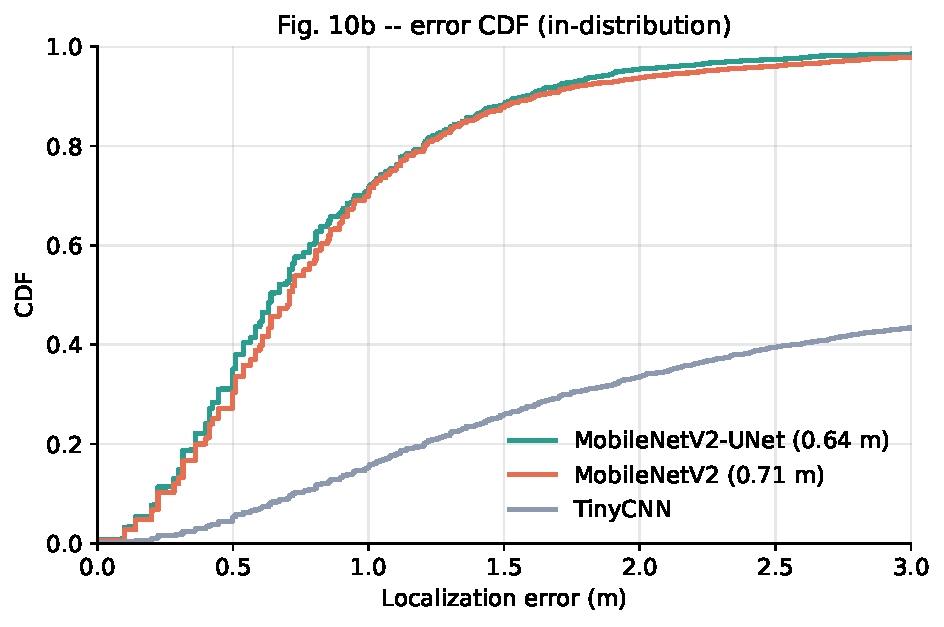
\includegraphics[width=0.74\linewidth]{cdf_fig10b}
\caption{In-distribution error CDF. Read it as: at each distance on the $x$-axis, what fraction of
predictions are at least that accurate ($y$-axis). The MobileNetV2-UNet dominates (up and to the
left); TinyCNN, starved of capacity, never reaches the $0.8$ level within 3\,m.}
\label{fig:eval:cdf}
\end{figure}

\section{The pixel-quantization gotcha}
\label{sec:eval:quant}

Here is a trap that the thesis is careful about and a committee may probe. Because the error is a
\emph{pixel} distance scaled by $0.1$, and pixel offsets are integers, the achievable error values are
\emph{quantized}: they can only be multiples of $0.1\sqrt{n}$ for integer $n$ (since
$\sqrt{\Delta x^2 + \Delta y^2}$ with integer $\Delta x,\Delta y$ takes only discrete values
$0,\,1,\,\sqrt2,\,2,\,\sqrt5,\dots$). One consequence is decisive:

\begin{keyidea}
Two models can report the \emph{identical} median (e.g.\ several of ours sit exactly at $0.707$ or
$0.640$\,m) yet have genuinely different error \emph{distributions}. An identical median is sometimes
a quantization artifact, \emph{not} evidence that the models are equally good. This is precisely why
the thesis reports the mean, the percentiles, and the full CDF alongside the median ---and why you
should never argue a result from the median alone.
\end{keyidea}

\section{Robustness corruptions}
\label{sec:eval:corruptions}

Robustness is measured by \emph{corrupting the CSI input at test time only} ---the models are
\textbf{not} retrained ---and re-measuring the error. Each corruption simulates a real-world failure:
\begin{description}[leftmargin=2.0cm,style=nextline,nosep]
  \item[AP dropout] Zero out one AP's channel, either a specific AP or a random one (and random
  2-AP dropout). Simulates an access point failing or going out of range.
  \item[Gaussian noise $\sigma\in\{0.1,0.2\}$] Add random noise to the CSI. Simulates interference and
  low signal-to-noise conditions.
  \item[Global attenuation $0.5\times$] Halve the whole signal. Simulates overall signal weakening.
  \item[Single-AP attenuation $0.3\times$] Drop one AP's strength to $30\%$. Simulates one weak or
  distant AP.
  \item[Blur ($5\times5$, $\sigma{=}1$)] Gaussian-blur the CSI heatmap. Simulates loss of spatial
  sharpness / lower effective bandwidth.
\end{description}
Testing without retraining is the strict choice: it measures how a \emph{deployed} model copes with
conditions it never saw, rather than how well it can be trained to anticipate them. (Training-time
corruption augmentation is left to future work.)

\section{Cross-session protocols: the fair one and the ablation}
\label{sec:eval:crosssession}

``Cross-session'' means testing in a different data-collection session than you trained on ---the
realistic case where the environment changes over time. The thesis runs \emph{two} protocols, and
keeping them straight is essential because only one is a fair comparison to DLoc.

\begin{description}[leftmargin=1.6em,style=nextline,nosep]
  \item[Leave-one-session-out (LOSO) --- the fair comparison.] Three folds; each fold holds out one
  August session and trains on the remaining setups, then tests on the held-out session. We run the
  MobileNetV2-UNet over three random seeds per fold. This \emph{exactly matches the protocol used to
  report the published DLoc numbers}, so the comparison in Section~\ref{ch:arch} is apples-to-apples.
  Because re-distilling would require retraining a teacher per fold, the LOSO models are
  \textbf{standalone only}.
  \item[Zero-shot stress test --- an internal ablation.] Train on \emph{only} the two July sessions
  and evaluate on the August sessions. This deliberately uses less training data and is \textbf{not} a
  fair DLoc comparison; it exists to compare \emph{our own} architectures and the effect of
  distillation against each other under a harder shift.
\end{description}

\begin{defensetip}
If a committee member compares our cross-session numbers to DLoc, make sure they are looking at the
\textbf{LOSO} table (mean $0.930$\,m vs DLoc $0.86$\,m), not the zero-shot table. Conflating the two
understates the model. The zero-shot numbers answer a different question (``does distillation help
under a bigger shift?'' ---yes, but only on the hardest fold).
\end{defensetip}

\section{The session difficulty hierarchy}
\label{sec:eval:sessions}

The WILD dataset has five sessions (Table~\ref{tab:eval:sessions}). They are not equally hard: errors
rise monotonically from the furniture sessions to the reflector session, a property of the
\emph{environment}, not of any model. The aluminum-reflector session is hardest because it injects
strong \emph{specular multipath} ---mirror-like reflections that create convincing ``phantom''
locations.

\begin{table}[H]
\centering
\caption{The five WILD collection sessions (Jacobs Hall, UC San Diego, 4 APs).}
\label{tab:eval:sessions}
\begin{tabular}{@{}llrl@{}}
\toprule
\textbf{Session} & \textbf{Tag} & \textbf{Samples} & \textbf{Condition} \\
\midrule
1 & \code{jacobs\_Jul28}        & ---     & training (reference conditions) \\
2 & \code{jacobs\_Jul28\_2}     & 4{,}260$^\dagger$ & in-distribution test (1\,h later, identical) \\
3 & \code{jacobs\_Aug16\_1}     & 11{,}201 & furniture rearrangement \\
4 & \code{jacobs\_Aug16\_3}     & 8{,}754  & different furniture configuration \\
5 & \code{jacobs\_Aug16\_4\_ref}& 5{,}486  & aluminum reflector (specular multipath) \\
\bottomrule
\end{tabular}

\vspace{0.3em}
{\footnotesize $^\dagger$ Held-out test split; Sessions~1+2 together provide 17{,}574 training
samples. Sessions 3--5 were collected three weeks later with deliberate environmental changes.}
\end{table}

\section{Computational efficiency metrics}
\label{sec:eval:efficiency}

Finally, deployment cost is measured four ways (reported in the thesis's efficiency table):
\begin{description}[leftmargin=1.8cm,style=nextline,nosep]
  \item[Parameters] The model's memory footprint ---how much storage/RAM the weights need.
  \item[FLOPs] Floating-point operations for one forward pass (batch size 1, dummy input). The
  compute cost per prediction.
  \item[CPU latency] Wall-clock time for one prediction on a CPU ---\textbf{the number that matters
  most for edge deployment}, since most gateways and APs have no GPU.
  \item[GPU latency] Wall-clock time on a GPU, for completeness.
\end{description}
The punchline you will need cold: the MobileNetV2-UNet runs in $27.2$\,ms on CPU and $1.45$\,GFLOPs,
versus DLoc's $270.9$\,ms and $81.06$\,GFLOPs ---a $10\times$ latency and $56\times$ compute reduction
at \emph{better} accuracy. That combination is the whole case for edge deployment.

%% ====================================================================
%%  Chapter 5 — The Architectures, Model by Model
%% ====================================================================
\chapter{The Architectures, Model by Model}
\label{ch:arch}

This is the heart of the guide. Each of the five models is dissected in the same five steps:
\emph{(1)} at a glance, \emph{(2)} the architecture, \emph{(3)} the concepts it embodies (pointing
back to Chapter~\ref{ch:blocks}), \emph{(4)} its results, and ---most importantly---
\emph{(5) why it behaved that way}. Read horizontally if you want one model cold; read vertically (all
the ``why'' boxes) if you want the comparison. Table~\ref{tab:arch:summary} is the map.

\begin{table}[H]
\centering
\footnotesize
\setlength{\tabcolsep}{5pt}
\caption{The five models at a glance. ``Compression'' is relative to the 16.5\,M DLoc teacher.}
\label{tab:arch:summary}
\begin{tabular}{@{}lrrll@{}}
\toprule
\textbf{Model} & \textbf{Params} & \textbf{Compr.} & \textbf{In-dist median} & \textbf{One-line verdict} \\
\midrule
DLoc (teacher)   & 16.5M & $1\times$    & 0.707\m\ (repro) & accurate but heavy; the thing we compress \\
MobileNetV2      & 2.3M  & $7.2\times$  & 0.707\m          & lossless compression; noise-fragile alone \\
TinyCNN          & 47K   & $351\times$  & 3.922\m          & below the capacity floor; KD \emph{harms} it \\
MobileNetV2-UNet & 2.41M & $6.8\times$  & \best{0.640\m}   & \best{beats the teacher}; best robustness \\
Mamba            & 0.65M & $25\times$   & \worst{10.56\m}  & architectural mismatch; the negative result \\
\bottomrule
\end{tabular}
\end{table}

%% ===================================================================
\section{DLoc --- the teacher and baseline}
\label{sec:arch:dloc}

\begin{ataglance}{DLoc}
\textbf{Role:} teacher (for distillation) \emph{and} accuracy/efficiency baseline.\quad
\textbf{Params:} 16.5\,M.\quad \textbf{Compression:} $1\times$ (the reference).\quad
\textbf{Verdict:} sub-meter accurate, but three heavy ResNet stacks make it unfit for the edge ---the
problem the thesis exists to solve.
\end{ataglance}

\paragraph{The architecture.} DLoc is an \emph{encoder with two decoders} (\code{Enc\_2Dec\_Network}),
in the style of image-translation generators. A shared \textbf{ResNet encoder} (a $7\times7$ input
convolution $4\to64$, two stride-2 downsamples $64\to128\to256$, then \textbf{6 residual blocks} at
the bottleneck, $64$ base filters) compresses the four-channel input. Two decoders then read that
shared latent:
\begin{itemize}[leftmargin=1.4em,nosep]
  \item a \textbf{location decoder} (9 residual blocks $+$ transposed-convolution upsampling $+$ a
  $7\times7$ output conv to 1 channel) that produces the location heatmap; and
  \item a \textbf{consistency (offset) decoder} (12 residual blocks, 4 output channels) that
  reproduces the offset-free per-AP heatmaps (\code{features\_wo\_offset}).
\end{itemize}
All normalization is InstanceNorm; training uses Adam ($\beta_1{=}0.5$, lr~$10^{-5}$, no annealing in
the original paper), batch size~32. At \emph{inference}, only the location decoder is used: the
prediction is its heatmap's argmax.

\paragraph{Concepts it embodies.} Residual/skip connections (Sec.~\ref{sec:blocks:resnet}) and the
encoder--decoder skeleton (Sec.~\ref{sec:blocks:encdec}). Its defining idea is the
\textbf{consistency decoder}: because each AP's input carries an unknown clock offset
(Sec.~\ref{sec:found:offset}), forcing the network to predict per-AP heatmaps that \emph{agree} across
all four APs teaches it to (i) remove the offset, (ii) resolve multipath by picking the direct path,
and (iii) sharpen low-bandwidth inputs (super-resolution). One AP cannot disambiguate its own offset;
four mutually consistent APs can.

\paragraph{Its results.} In our reproduction, DLoc reaches a median of \textbf{0.707\,m} in
distribution (the published paper reports 0.64\,m; the gap is an implementation difference, discussed
below). Under the fair leave-one-session-out protocol the \emph{published} DLoc averages 0.86\,m. Our
multi-seed reproduction of the baseline gives a median of $0.875 \pm 0.036$\,m over three seeds ---low
seed-to-seed variance (coefficient of variation $4.1\%$), confirming the baseline is stable. Its cost
is the headline problem: \textbf{16.5\,M parameters, 81.06\,GFLOPs, 270.9\,ms} on CPU.

\begin{whybox}
DLoc is \emph{accurate} because its dual-decoder design directly attacks the physics: the consistency
decoder resolves the clock offset and multipath that defeat classical geometry, and 16.5\,M parameters
give it ample capacity. It is \emph{heavy} because it stacks \emph{three} ResNet towers (encoder $+$
two decoders) at 64 base filters. Crucially, most of that capacity is wasted in distribution ---the
next model matches DLoc's accuracy with $7.2\times$ fewer parameters, which is the thesis's founding
evidence that DLoc is \textbf{over-parameterized}, not fundamentally large.
\end{whybox}

%% ===================================================================
\section{MobileNetV2 --- lossless compression}
\label{sec:arch:mobilenet}

\begin{ataglance}{MobileNetV2}
\textbf{Role:} the ``can we just shrink it?'' student.\quad \textbf{Params:} 2.3\,M.\quad
\textbf{Compression:} $7.2\times$.\quad \textbf{Verdict:} matches the DLoc baseline median
\emph{exactly} in distribution ---but, trained standalone, it is alarmingly fragile to noise.
\end{ataglance}

\paragraph{The architecture.} Replace DLoc's ResNet encoder with a \textbf{MobileNetV2 backbone}
(depthwise-separable convolutions in inverted-residual blocks), with the first convolution adapted to
accept the four CSI channels. A lightweight decoder head maps the backbone's features to the
single-channel heatmap. About \textbf{2.3\,M} parameters.

\paragraph{Concepts it embodies.} Depthwise-separable convolutions
(Sec.~\ref{sec:blocks:dwsep}) and inverted residuals with linear bottlenecks
(Sec.~\ref{sec:blocks:invres}) ---the efficiency trick that buys the $7.2\times$ shrink--- on the same
encoder--decoder skeleton. Notably it has \emph{no} skip connections to the decoder and \emph{no}
consistency decoder.

\paragraph{Its results.} In distribution it reaches \textbf{0.707\,m} ---identical to the DLoc
baseline--- with P90~$1.616$ and P99~$3.992$. Standalone and distilled medians are the same. The
robustness story is where it gets interesting:
\begin{itemize}[leftmargin=1.4em,nosep]
  \item Under Gaussian noise ($\sigma{=}0.1$) the \emph{standalone} model collapses to a
  \worst{16.368\,m} median ---effectively guessing--- while the \emph{distilled} model holds at
  \best{4.769\,m}, a $\mathbf{3.4\times}$ improvement.
  \item Under random 2-AP dropout it degrades gracefully to $\sim$2.4--2.5\,m; under $0.5\times$
  attenuation, $\sim$1.3--1.5\,m; under blur, $\sim$0.85\,m.
\end{itemize}
Efficiency: \textbf{2.27\,M params, 1.28\,GFLOPs, 17.9\,ms} CPU.

\begin{whybox}
\textbf{Why lossless in distribution:} depthwise-separable convolutions preserve nearly all of a
standard convolution's representational power, so 2.3\,M parameters suffice to learn the clean
CSI$\to$location mapping ---DLoc's extra 14\,M were redundant here. \textbf{Why so noise-fragile when
standalone:} MobileNetV2 squeezes everything through an aggressive low-dimensional bottleneck and
keeps \emph{no} shallow, high-resolution shortcut. A small noise perturbation scrambles that single
latent, and with no alternative path the predicted peak jumps far away ($16.4$\,m). \textbf{Why
distillation rescues it:} matching the teacher's soft, spread-out heatmap (Ch.~\ref{ch:distill})
regularizes the encoder toward smoother, more noise-tolerant features ---spatial label smoothing in
action--- recovering it to $4.8$\,m. This is the cleanest single demonstration that, here, distillation
is a \emph{robustness} lever, not an accuracy lever.
\end{whybox}

%% ===================================================================
\section{TinyCNN --- below the capacity floor}
\label{sec:arch:tinycnn}

\begin{ataglance}{TinyCNN}
\textbf{Role:} a deliberate probe of ``how small is too small?''\quad \textbf{Params:} 47\,K.\quad
\textbf{Compression:} $351\times$.\quad \textbf{Verdict:} too small to learn the task ($\sim$5$\times$
worse than baseline), and the one model that distillation actively \emph{harms}.
\end{ataglance}

\paragraph{The architecture.} A minimal network: \textbf{three convolutional layers and two
fully-connected layers}, $\approx$\textbf{47{,}000} parameters. No skips, no depthwise tricks, no
second decoder ---intentionally bare-bones.

\paragraph{Concepts it embodies.} Only the most basic convolution (Sec.~\ref{sec:blocks:conv}) plus a
fully-connected head. It is the control that defines the bottom of the size axis.

\paragraph{Its results.} In distribution it reaches \textbf{3.922\,m} (standalone) / 3.706\,m
(distilled) ---about five times the baseline error--- with P90~$\approx$14\,m. Under corruption,
distillation makes it \emph{worse}, not better:
\begin{itemize}[leftmargin=1.4em,nosep]
  \item random 1-AP dropout: $7.940\to\worst{13.648}$\,m (standalone $\to$ distilled);
  \item $0.5\times$ attenuation: $9.708\to\worst{18.532}$\,m.
\end{itemize}
Efficiency is trivially cheap (47\,K params, 0.66\,GFLOPs, 9.1\,ms) ---but useless at this accuracy.

\begin{whybox}
\textbf{Why it fails outright:} the CSI$\to$location task requires learning \emph{both} per-AP signal
features \emph{and} how to fuse four APs into one spatial estimate. With only 47\,K parameters the
model is below the task's \textbf{capacity floor} ($\sim$2\,M, per the thesis), so no amount of
training reaches sub-meter accuracy. \textbf{Why distillation \emph{harms} it:} a tiny model has no
spare capacity. Forced to also imitate the teacher's modeled \emph{AP interactions}, it spends its
scarce parameters memorizing those interactions ---which become \emph{invalid} the instant an AP is
dropped at test time, leaving nothing to fall back on. This is the lower edge of the capacity-threshold
finding (Ch.~\ref{ch:findings}): distillation only helps a student rich enough to absorb the teacher's
hints \emph{without} sacrificing its own robustness.
\end{whybox}

%% ===================================================================
\section{MobileNetV2-UNet --- the model that beats its teacher}
\label{sec:arch:unet}

\begin{ataglance}{MobileNetV2-UNet}
\textbf{Role:} the headline model and practical recommendation.\quad \textbf{Params:} 2.41\,M.\quad
\textbf{Compression:} $6.8\times$.\quad \textbf{Verdict:} \best{better accuracy than the 16.5\,M
teacher} (0.640 vs 0.707\,m), the best robustness of any student, and cross-session accuracy
competitive with published DLoc.
\end{ataglance}

\paragraph{The architecture.} Take the MobileNetV2 encoder and add \textbf{U-Net skip connections}
into the decoder (Figure~\ref{fig:arch:unet}). The encoder runs in stages of $32\to24\to32\to96\to320$
channels; the decoder upsamples and \emph{concatenates} the matching-resolution encoder features
before each block: $320{+}96\to128$ (dec1), $128{+}32\to64$ (dec2), $64{+}24\to32$ (dec3), then a
$1\times1$ convolution and sigmoid head to one channel. Trained for 120 epochs (Adam, lr~$10^{-4}$,
cosine or step-decay schedule), standalone and distilled.

\begin{figure}[H]
\centering
\resizebox{\linewidth}{!}{% ============================================================================
%  MobileNetV2-UNet architecture — \input-able body (no \documentclass).
%  Requires in the master preamble: \usepackage{tikz} and
%  \usetikzlibrary{positioning, arrows.meta, calc}.  Colours are defined here
%  so the figure is self-contained.  Layer specs from code/models/student_unet.py.
% ============================================================================
\definecolor{cEnc}{RGB}{142,202,230}
\definecolor{cBottle}{RGB}{33,102,172}
\definecolor{cDec}{RGB}{69,123,157}
\definecolor{cHead}{RGB}{188,108,37}
\definecolor{cSkip}{RGB}{42,157,143}
\definecolor{cIO}{RGB}{230,57,70}

\begin{tikzpicture}[
  font=\small,
  >={Stealth[length=2.4mm]},
  block/.style={rectangle, rounded corners=2pt, draw=black!70, thick,
                minimum height=11mm, minimum width=13mm, align=center,
                text=white, font=\footnotesize\bfseries},
  enc/.style={block, fill=cEnc, text=black},
  bottle/.style={block, fill=cBottle},
  dec/.style={block, fill=cDec},
  head/.style={block, fill=cHead},
  io/.style={rectangle, rounded corners=1pt, draw=black!70, thick,
             minimum height=13mm, minimum width=12mm, align=center,
             fill=cIO!12, font=\footnotesize},
  flow/.style={->, black!75, thick},
  skipline/.style={->, cSkip, very thick, dashed},
]
\node[io] (in) {Input\\$4{\times}161{\times}361$};
\node[enc,    right=7mm of in]  (inc) {inc\\$4{\to}32$\\/2};
\node[enc,    right=6mm of inc] (e1)  {enc1\\$24$};
\node[enc,    right=6mm of e1]  (e2)  {enc2\\$32$};
\node[enc,    right=6mm of e2]  (e3)  {enc3\\$96$};
\node[bottle, right=6mm of e3]  (e4)  {enc4\\$320$};
\node[dec,  right=11mm of e4] (d1) {dec1\\$416{\to}128$};
\node[dec,  right=6mm of d1]  (d2) {dec2\\$160{\to}64$};
\node[dec,  right=6mm of d2]  (d3) {dec3\\$88{\to}32$};
\node[head, right=6mm of d3]  (hd) {head\\$32{\to}1$\\Sigmoid};
\node[io,   right=7mm of hd]  (out) {Output\\$1{\times}161{\times}361$};
\draw[flow] (in)--(inc); \draw[flow] (inc)--(e1); \draw[flow] (e1)--(e2);
\draw[flow] (e2)--(e3);  \draw[flow] (e3)--(e4);  \draw[flow] (e4)--(d1);
\draw[flow] (d1)--(d2);  \draw[flow] (d2)--(d3);  \draw[flow] (d3)--(hd);
\draw[flow] (hd)--(out);
\draw[skipline] (e3.north) to[out=90,in=90]
      node[above,font=\tiny,text=cSkip]{skip 96} (d1.north);
\draw[skipline] (e2.north) to[out=90,in=90]
      node[above,font=\tiny,text=cSkip]{skip 32} (d2.north);
\draw[skipline] (e1.north) to[out=90,in=90]
      node[above,font=\tiny,text=cSkip]{skip 24} (d3.north);
\node[text=black!60, font=\scriptsize, below=3mm of e2.south] {MobileNetV2 encoder (pretrained, 4-ch input)};
\node[text=black!60, font=\scriptsize, below=3mm of d2.south] {U-Net decoder (upsample $+$ skip concat)};
\end{tikzpicture}
}
\caption{The MobileNetV2-UNet. A MobileNetV2 encoder (light blue) downsamples the four-channel CSI
input; a decoder (dark blue) upsamples back to full resolution; teal dashed arcs are the U-Net skip
connections that concatenate encoder feature maps into the decoder at matching resolutions, bypassing
the bottleneck (deep blue). Layer specs are exact, from \code{code/models/student\_unet.py}.}
\label{fig:arch:unet}
\end{figure}

\paragraph{Concepts it embodies.} Everything MobileNetV2 has (depthwise-separable convolutions,
inverted residuals) \emph{plus} U-Net skip connections (Sec.~\ref{sec:blocks:unet}). It deliberately
\emph{omits} DLoc's consistency decoder ---a single-decoder design--- which matters on the reflector
fold below.

\paragraph{Its results.} The best of every student:
\begin{itemize}[leftmargin=1.4em,nosep]
  \item \textbf{In distribution:} \best{0.640\,m} median ---a $9.5\%$ improvement over both DLoc and
  plain MobileNetV2--- with P90~$1.513$ and P99~$2.587$ (distilled, cosine). The learning-rate
  schedule barely matters (cosine's tails are slightly tighter than step-decay's); the
  \emph{architecture} dominates.
  \item \textbf{Robustness:} standalone, it holds \best{3.000\,m} under $\sigma{=}0.1$ noise versus
  plain MobileNetV2's 16.368\,m ---a $\mathbf{5.5\times}$ improvement from the skips alone. Distillation
  separately helps most under \emph{multi-AP dropout} (random 2-AP: $3.324\to\best{2.730}$\,m).
  \item \textbf{Cross-session (LOSO, 3 seeds):} medians of $0.852$, $0.822$, $1.116$\,m on the three
  held-out August folds, averaging \textbf{0.930\,m} against published DLoc's 0.86\,m ---and matching
  DLoc on the different-furniture fold ($0.822$ vs $0.82$\,m) and beating it on the reflector P90
  ($2.489$ vs $2.77$\,m). Standard deviations are tiny ($0.016$--$0.044$\,m).
  \item \textbf{Efficiency:} 2.41\,M params, \textbf{1.45\,GFLOPs, 27.2\,ms} CPU ---$56\times$ fewer
  FLOPs and $10\times$ less CPU latency than DLoc.
\end{itemize}
Its 0.640\,m median is \textbf{6.5 standard deviations} below the baseline's $0.875\pm0.036$\,m mean
---a statistically unambiguous improvement, not seed luck.

\begin{figure}[H]
\centering
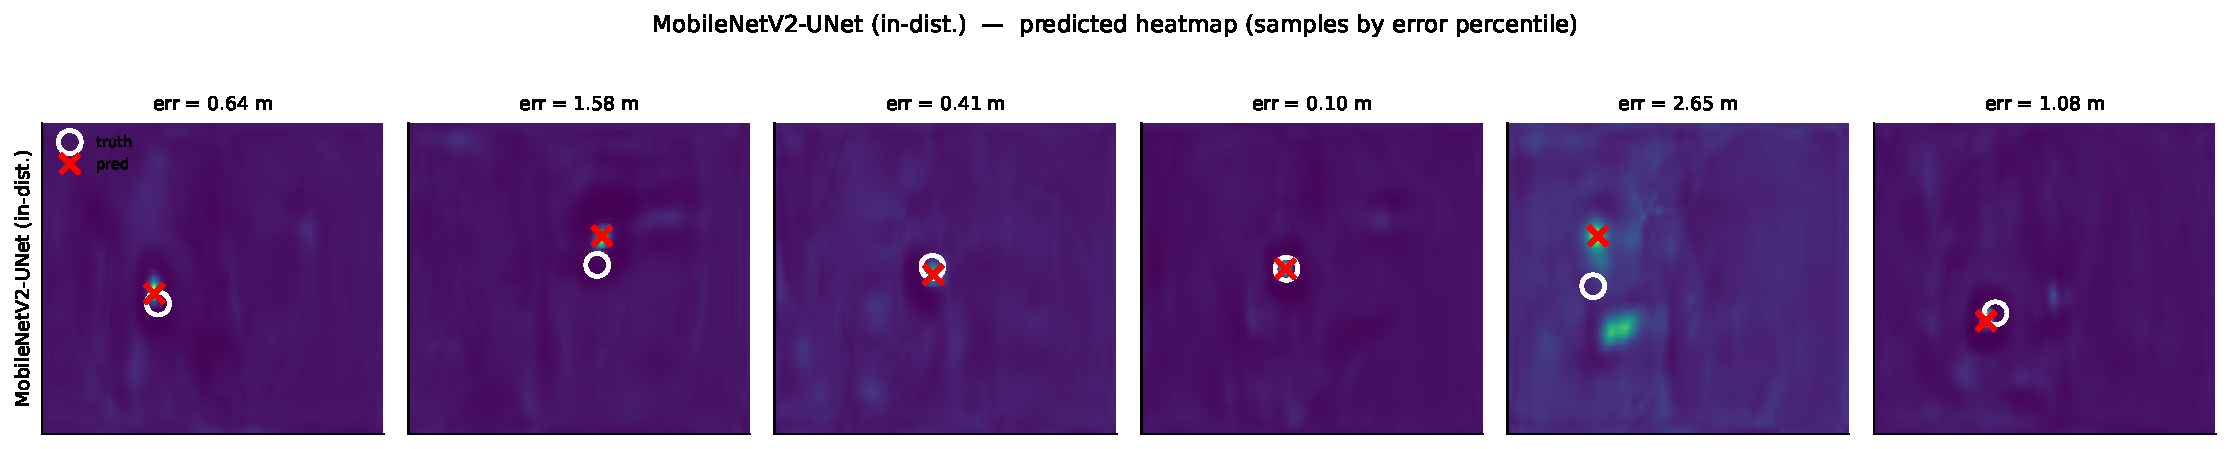
\includegraphics[width=\linewidth]{heatmaps_unet_fig10b}
\caption{Qualitative in-distribution predictions of the MobileNetV2-UNet. Each panel is a test sample
at a given error percentile; the white circle marks the ground-truth peak and the red cross the
prediction. Low-error cases (left) are tight and single-mode; the high-error case is multimodal, with
the chosen peak displaced.}
\label{fig:arch:hm_indist}
\end{figure}

\begin{whybox}
\textbf{Why it beats the teacher:} the skip connections feed the decoder the \emph{high-resolution
spatial detail} that the bottleneck throws away (Sec.~\ref{sec:blocks:unet}). Since the answer
\emph{is} a precise spatial location, restoring that detail directly lowers the error ---0.640 beats
DLoc's 0.707 with $6.8\times$ fewer parameters. \textbf{Why it is so noise-robust:} those same shallow
features travel a short path that bypasses the noise-amplifying bottleneck, so a corrupted latent no
longer dooms the prediction ($5.5\times$ better than plain MobileNetV2) ---an \emph{architectural}
robustness, independent of distillation. \textbf{Why it trails slightly on the reflector median:} it
has no consistency decoder to enforce cross-AP agreement, and that mechanism is exactly what helps most
under the aluminum reflector's strong specular multipath; the qualitative heatmaps there show extra
``phantom'' probability mass. Even so it still wins the reflector \emph{P90}, so the gap is small and
confined to the hardest fold.
\end{whybox}

\begin{figure}[H]
\centering
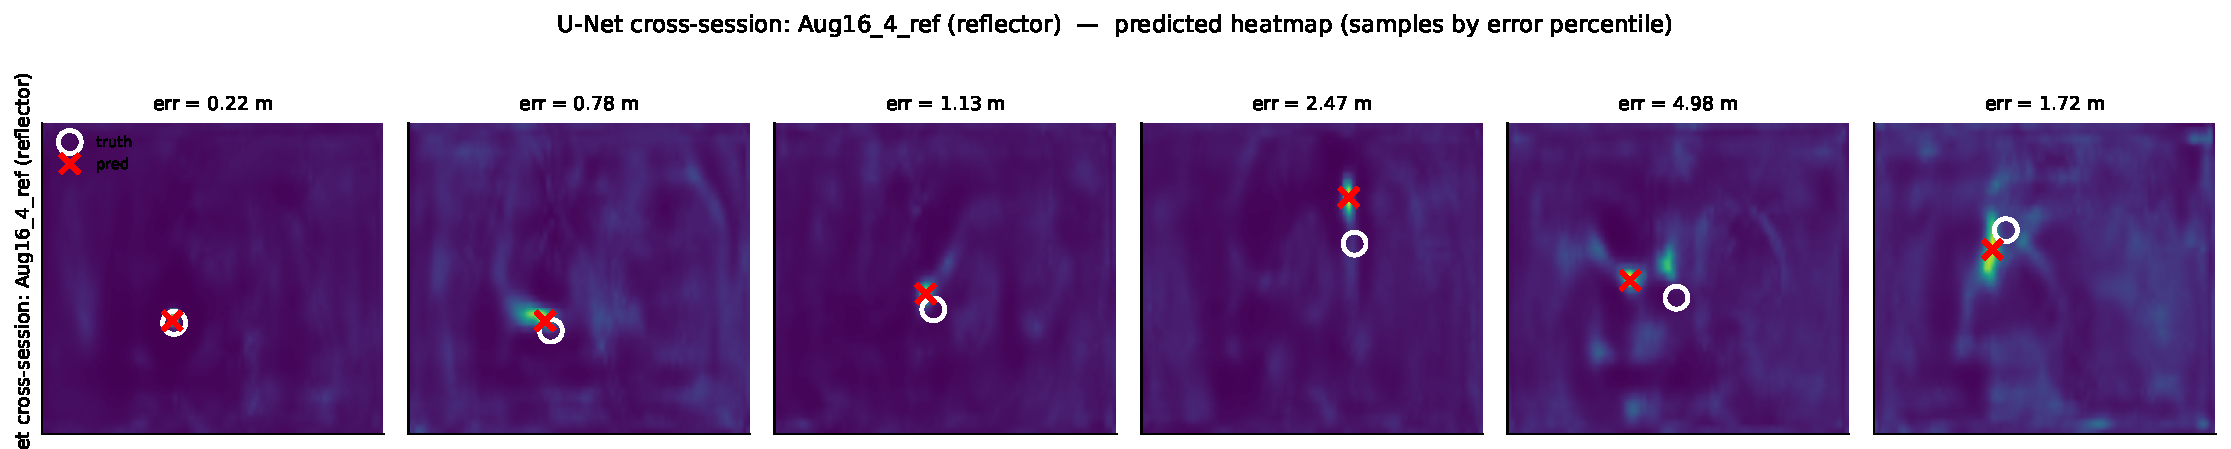
\includegraphics[width=\linewidth]{heatmaps_unet_cross_env4}
\caption{Qualitative cross-session predictions on the reflector fold (Aug16\_4\_ref). Compared with the
in-distribution panels of Figure~\ref{fig:arch:hm_indist}, the heatmaps carry extra scattered
probability mass ---the specular ``phantom'' reflections from the aluminum panel--- which drives the
larger errors on this fold and is exactly what the absent consistency decoder would suppress.}
\label{fig:arch:hm_reflector}
\end{figure}

%% ===================================================================
\section{Mamba --- the instructive negative result}
\label{sec:arch:mamba}

\begin{ataglance}{Mamba}
\textbf{Role:} a deliberately different inductive bias.\quad \textbf{Params:} 0.65\,M.\quad
\textbf{Compression:} $25\times$.\quad \textbf{Verdict:} fails to learn the task (worst median of all),
and the failure is \emph{diagnostic} ---it isolates why the image framing matters.
\end{ataglance}

\paragraph{The architecture.} A \textbf{selective state-space (Mamba) model}
(Sec.~\ref{sec:blocks:mamba}) with $\approx$0.65\,M parameters. Unlike every other model, it does
\emph{not} treat the CSI as a 2D image; it flattens each AP's measurements into a \textbf{1D sequence}
and processes them with a recurrent state.

\paragraph{Concepts it embodies.} State-space sequence modeling with a content-selective recurrence.
Its whole reason for existence is to test whether a non-convolutional, sequence-style inductive bias
can compete on the CSI-to-heatmap problem.

\paragraph{Its results.} It reaches a median of \worst{10.56\,m} (P90~$20.0$, P99~$28.3$) ---the worst
of any model, placing it at the unfavorable top of the accuracy--size plane. Tellingly, it achieves
its \emph{best} accuracy at the very first epoch and then degrades \emph{monotonically}, with training
and test error rising \emph{together}.

\begin{whybox}
\textbf{Why it fails ---and why it is \emph{not} a capacity problem:} at 0.65\,M parameters Mamba is
larger than the 47\,K TinyCNN, yet far worse, so size is not the issue. The cause is an
\textbf{architectural mismatch}. The target is an inherently 2D spatial heatmap, but an SSM consumes a
1D ordered sequence; flattening the grid imposes an arbitrary scan order that \emph{destroys spatial
locality} ---pixels that are physical neighbors land far apart in the sequence. \textbf{Why we know it
is mismatch, not overfitting:} in overfitting, training error falls while test error rises. Here both
rise together after epoch~1, so the model is not memorizing the data; the selective state-space bias
is simply ill-suited to the problem. The result is kept because a clean negative result is itself
evidence: it confirms that the image-to-image \emph{framing} (Sec.~\ref{sec:found:translation}), not
merely ``a small modern network,'' is what makes the other students work.
\end{whybox}

\section{Reading the five together}
\label{sec:arch:together}

Lined up, the five models tell one story along the size axis. DLoc shows the task is solvable but
over-provisions capacity. MobileNetV2 strips that capacity away \emph{losslessly}, proving the excess
was redundant. TinyCNN strips \emph{too} much and falls through the capacity floor. The
MobileNetV2-UNet adds back the \emph{right} thing ---skip connections, not raw parameters--- and
overtakes the teacher. Mamba changes the \emph{framing} instead of the size and breaks, isolating the
image assumption as load-bearing. Chapter~\ref{ch:findings} turns these five vertical stories into the
six horizontal findings of the thesis.

%% ====================================================================
%%  Chapter 6 — Cross-Cutting Findings
%% ====================================================================
\chapter{Cross-Cutting Findings}
\label{ch:findings}

Chapter~\ref{ch:arch} told each model's own story. This chapter does the opposite: it states the six
findings that only emerge when you \emph{compare} models, and names the mechanism behind each. These
are the claims the thesis stakes, and the ones a committee will press on.

\section{Finding 1 --- Order-of-magnitude compression is lossless in distribution}
\label{sec:find:1}

\textbf{Claim.} A model with $7.2\times$ fewer parameters than DLoc reaches the \emph{same}
in-distribution accuracy. \textbf{Evidence.} Plain MobileNetV2 (2.3\,M) matches the DLoc baseline's
0.707\,m median exactly. \textbf{Mechanism.} Depthwise-separable convolutions retain a standard
convolution's representational power at a fraction of the cost, so DLoc's extra $\sim$14\,M parameters
were redundant for the clean mapping. \textbf{So what.} This is the founding result: DLoc is
\emph{over-parameterized}, not intrinsically large ---which is what licenses the entire compression
program.

\section{Finding 2 --- Architecture, not parameters, beats the teacher}
\label{sec:find:2}

\textbf{Claim.} A 2.41\,M student \emph{outperforms} the 16.5\,M teacher. \textbf{Evidence.} The
MobileNetV2-UNet reaches 0.640\,m, a $9.5\%$ improvement over DLoc's 0.707\,m at $6.8\times$ fewer
parameters; the gain is $6.5$ standard deviations beyond the baseline's seed-to-seed spread
($0.875\pm0.036$\,m), so it is real, not luck. \textbf{Mechanism.} U-Net skip connections restore the
high-resolution spatial detail the bottleneck discards ---and spatial detail is the answer. \textbf{So
what.} You buy accuracy with the \emph{right structure}, not with raw capacity; adding parameters (as
DLoc does) is the wrong lever.

\begin{figure}[H]
\centering
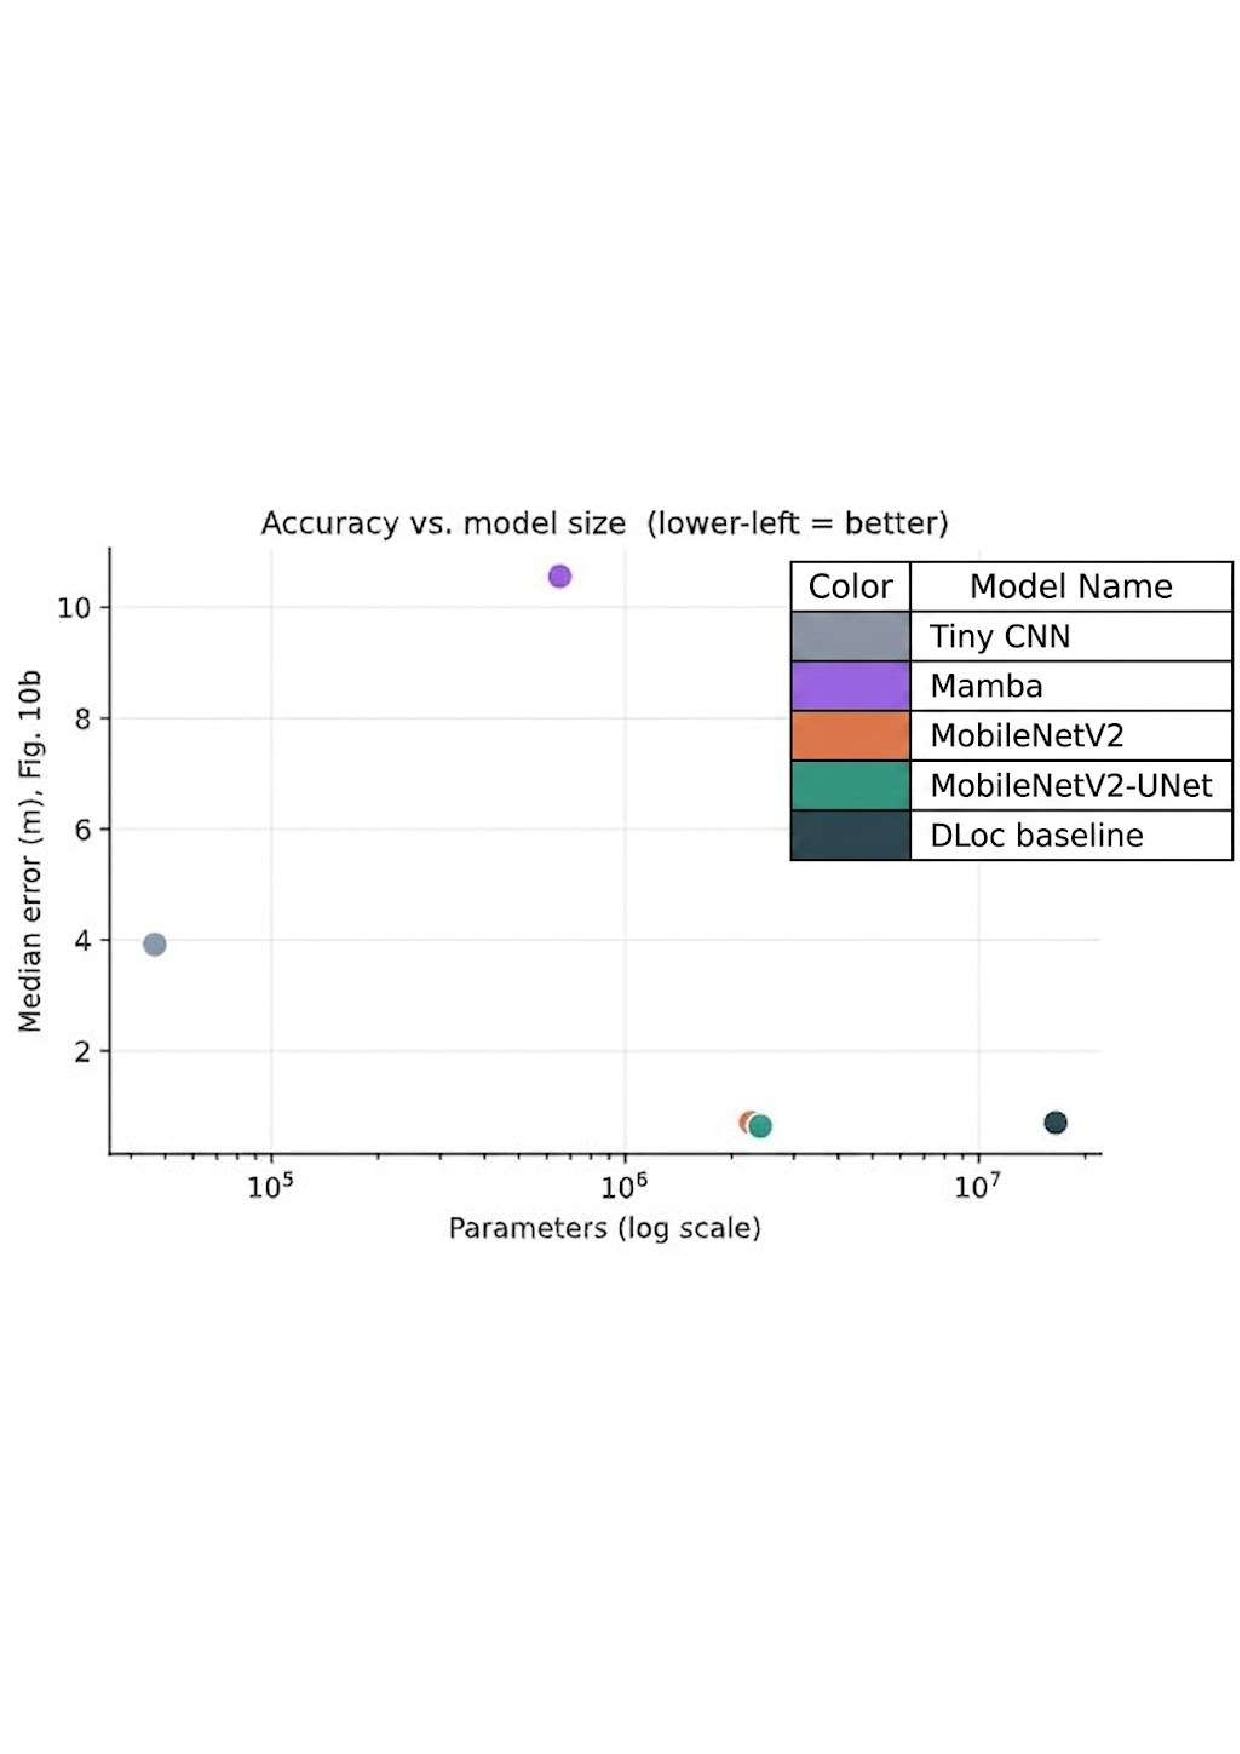
\includegraphics[width=0.66\linewidth]{compression_pareto}
\caption{Accuracy versus model size. The MobileNetV2-UNet sits at the favorable lower-left ---the best
median error of any model at a fraction of DLoc's parameters--- while Mamba (top) and TinyCNN mark the
two ways to fail: wrong framing and too little capacity.}
\label{fig:find:pareto}
\end{figure}

\section{Finding 3 --- Distillation buys robustness, not accuracy}
\label{sec:find:3}

\textbf{Claim.} In this heatmap task, knowledge distillation leaves clean accuracy unchanged but
sharply improves behavior under shift. \textbf{Evidence.} Standalone and distilled models share the
\emph{same} in-distribution median, yet distillation gives MobileNetV2 a $3.4\times$ better median
under $\sigma{=}0.1$ noise ($16.368\to4.769$\,m) and consistently helps on the hardest cross-session
fold. \textbf{Mechanism.} In distribution the teacher's soft heatmap is nearly identical to the ground
truth, so its term is redundant; off-distribution that ``spatial label smoothing'' regularizes the
student toward more tolerant features (Ch.~\ref{ch:distill}). \textbf{So what.} Distillation is worth
doing precisely for the realistic, degraded deployment case ---and judging it by clean accuracy alone
misses its entire value.

\section{Finding 4 --- Distillation has a capacity threshold ($\sim$2\,M)}
\label{sec:find:4}

\textbf{Claim.} Distillation helps only students above $\sim$2\,M parameters; below that it
\emph{hurts}. \textbf{Evidence.} It helps MobileNetV2 (2.3\,M) and MobileNetV2-UNet (2.41\,M) but
degrades TinyCNN (47\,K): under random 1-AP dropout TinyCNN worsens from 7.940 to 13.648\,m when
distilled. \textbf{Mechanism.} A tiny model has no spare capacity, so imitating the teacher's modeled
AP interactions crowds out its own fallback behavior; when an AP drops, those memorized interactions
become invalid. \textbf{So what.} Distillation is not free regularization ---it presupposes a student
rich enough to absorb the teacher's hints \emph{and} keep its own robustness.

\begin{keyidea}
Findings 3 and 4 together are the ``dual nature'' of distillation: the \emph{same} soft-target signal
\emph{regularizes} a large-enough student into robustness but \emph{overloads} a too-small one into
brittleness. One mechanism, two opposite outcomes, split at a capacity threshold.
\end{keyidea}

\section{Finding 5 --- The two robustness mechanisms are complementary, not additive}
\label{sec:find:5}

\textbf{Claim.} Skip connections and distillation each improve robustness, but against \emph{different}
corruptions, and stacking them does not simply add. \textbf{Evidence.} On the MobileNetV2-UNet, the
\emph{skips} dominate noise robustness (standalone $3.000$\,m at $\sigma{=}0.1$, a $5.5\times$ gain over
plain MobileNetV2), while \emph{distillation} dominates multi-AP dropout (random 2-AP:
$3.324\to2.730$\,m). Combining them under noise gives $3.469$\,m ---slightly \emph{worse} than the
standalone $3.000$, i.e.\ not additive. \textbf{Mechanism.} Skips provide an \emph{architectural} path
around a noisy bottleneck; distillation provides a \emph{training-time} feature regularizer. They
target different failure modes. \textbf{So what.} Choose the mechanism for the corruption you expect:
skips for high-noise environments, distillation for AP failures; do not assume both at once compounds.

\section{Finding 6 --- Cross-session accuracy is competitive for the cost}
\label{sec:find:6}

\textbf{Claim.} Under DLoc's own leave-one-session-out protocol, the compressed model is roughly on par
with published DLoc. \textbf{Evidence.} The MobileNetV2-UNet (3 seeds) reaches $0.852$, $0.822$,
$1.116$\,m on the three held-out August folds ---mean $0.930$\,m versus DLoc's $0.86$\,m. It
\emph{matches} DLoc on different-furniture ($0.822$ vs $0.82$), holds the \emph{same} average P90
($2.374$ vs $2.33$), and \emph{beats} DLoc's P90 on the reflector fold ($2.489$ vs $2.77$).
\textbf{Mechanism.} The skips generalize the spatial mapping well; the only soft spot is the reflector
median, where DLoc's consistency decoder helps most. \textbf{So what.} This is an honest
\emph{efficiency} result: near-DLoc generalization at $6.8\times$ fewer parameters, not a cross-session
accuracy win ---and the thesis states it that way.

\begin{figure}[H]
\centering
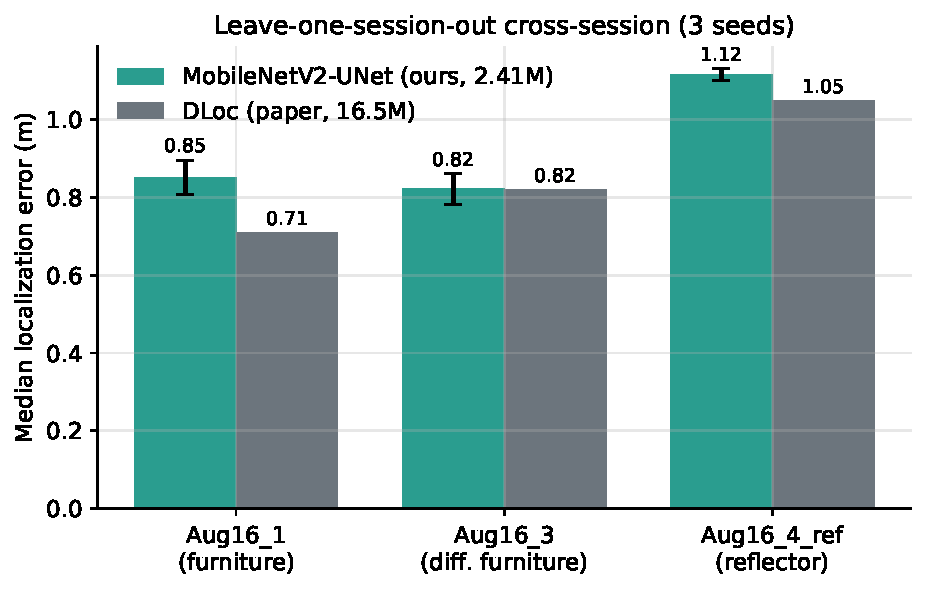
\includegraphics[width=0.7\linewidth]{crosssession_median}
\caption{Leave-one-session-out median error: our 2.41\,M MobileNetV2-UNet (three-seed mean $\pm$ std)
against the published 16.5\,M DLoc. The U-Net matches DLoc on the different-furniture fold and lands
within $\sim$0.1\,m on the others, at $6.8\times$ fewer parameters.}
\label{fig:find:crosssession}
\end{figure}

\begin{defensetip}
Frame Finding 6 carefully and you disarm the obvious challenge. Lead with ``competitive at $6.8\times$
compression,'' cite the fold it \emph{matches} and the P90 it \emph{beats}, and concede the small
reflector-median gap \emph{with its reason} (no consistency decoder). Honesty about the $\sim$0.07\,m
gap reads as rigor, not weakness.
\end{defensetip}

\section{The synthesis and the practical recommendation}
\label{sec:find:synthesis}

Put the six together and the thesis's answer to its own question ---``is DLoc's cost inherent?''--- is
a clear \emph{no}. A model an order of magnitude smaller can match or beat DLoc, provided you add the
right structure (skips) rather than parameters, and use distillation where capacity allows to harden
it against shift.

The practical recommendation that falls out:
\begin{itemize}[leftmargin=1.4em,nosep]
  \item \textbf{Default choice: distilled MobileNetV2-UNet.} Best in-distribution accuracy (0.640\,m),
  competitive cross-session, best under multi-AP dropout, and $56\times$ cheaper to run than DLoc.
  \item \textbf{If noise is the dominant threat:} the \emph{standalone} U-Net (its skips give the
  strongest noise robustness, which distillation slightly dilutes).
  \item \textbf{If raw compression is the only goal:} the distilled plain MobileNetV2 ---0.707\,m at
  just 2.3\,M parameters.
\end{itemize}
In every case, a model roughly an order of magnitude smaller than DLoc meets or exceeds its accuracy
---the single point the whole thesis is built to make.

%% ====================================================================
%%  Chapter 7 — Defense Q&A
%% ====================================================================
\chapter{Defense Q\&A}
\label{ch:qa}

This chapter rehearses the questions a committee is most likely to ask, grouped by topic, each with a
sharp answer and a pointer back to the concept that backs it up. Practice saying the answer in one or
two sentences first, then expand only if asked. When a number is involved, state it ---committees trust
specifics.

\section{Problem and framing}
\label{sec:qa:framing}

\textbf{Q1. Why predict a heatmap instead of directly regressing the $(x,y)$ coordinates?}\\
A heatmap preserves spatial structure and represents \emph{uncertainty} and \emph{multimodality}
---when two locations are plausible, the heatmap can show two bumps, and the argmax still gives a
decision. Direct coordinate regression collapses that structure, handles ambiguity poorly, and cannot
exploit the convolutional locality that makes the image framing work (Sec.~\ref{sec:found:translation}).

\textbf{Q2. What is CSI, and why does it carry location information?}\\
Channel State Information is the per-subcarrier, per-antenna complex channel estimate WiFi hardware
already computes. Amplitude is a (noisy) distance cue; phase progression \emph{across antennas} encodes
angle of arrival; phase progression \emph{across subcarriers} encodes time of flight, hence distance
(Sec.~\ref{sec:found:csi}--\ref{sec:found:aoa}).

\textbf{Q3. Why four input channels?}\\
One channel per access point; the Jacobs Hall environment has four APs, stacked into a
$[4,161,361]$ image at $0.1$\,m/pixel (Sec.~\ref{sec:found:aoa}).

\textbf{Q4. What is the clock/ToF offset and why does it matter?}\\
Device and AP clocks are unsynchronized, so an unknown delay shifts each AP's heatmap radially (by
$10$--$15$\,m) and the four APs disagree on the location. Resolving this is the core thing a
\emph{learned} system does and classical geometry cannot ---it is what DLoc's consistency decoder is for
(Sec.~\ref{sec:found:offset}).

\textbf{Q5. Why deep learning rather than a classical method like SpotFi?}\\
Classical AoA/ToF estimation degrades badly under non-line-of-sight and rich multipath, where the
strongest path is often a reflection. A network learns to pick the direct path by cross-checking APs
and to undo the offset, at the price of model size ---which is exactly what we then compress
(Sec.~\ref{sec:found:why_dl}).

\section{Architectures}
\label{sec:qa:arch}

\textbf{Q6. How can a 2.41\,M student beat its own 16.5\,M teacher?}\\
U-Net skip connections feed the decoder high-resolution spatial detail that the encoder bottleneck
discards; since the answer is a precise location, restoring that detail lowers error to 0.640\,m vs
0.707\,m. The improvement is $6.5$ standard deviations beyond the baseline's seed spread, so it is real
(Sec.~\ref{sec:arch:unet}, Finding~2).

\textbf{Q7. What are depthwise-separable convolutions, in one breath?}\\
A standard convolution mixes space and channels at once; the separable version splits it into a cheap
spatial mix (depthwise) and a cheap channel mix (pointwise, $1\times1$), cutting cost about
$8$--$9\times$ for nearly the same power. They are why 2.3\,M parameters suffice
(Sec.~\ref{sec:blocks:dwsep}).

\textbf{Q8. Why did TinyCNN fail?}\\
At 47\,K parameters it is below the task's $\sim$2\,M capacity floor; it cannot learn both per-AP signal
features and four-AP spatial fusion, so it lands at $\sim$3.9\,m, five times the baseline
(Sec.~\ref{sec:arch:tinycnn}).

\textbf{Q9. Why did Mamba fail ---and is that just because it is small?}\\
No: at 0.65\,M it is \emph{larger} than TinyCNN yet far worse, so it is not capacity. It is an
architectural mismatch ---Mamba consumes a 1D sequence, but the target is a 2D heatmap; flattening
destroys spatial locality. And it is not overfitting, because training and test error rise
\emph{together} after epoch~1 (Sec.~\ref{sec:arch:mamba}).

\textbf{Q10. What is the consistency decoder, and do your students have one?}\\
It is DLoc's second decoder, trained to make the four per-AP heatmaps agree; that agreement teaches
offset removal, multipath resolution, and super-resolution. Our students omit it (single-decoder
design), which is why they trail DLoc slightly on the reflector fold's median
(Sec.~\ref{sec:arch:dloc}, Sec.~\ref{sec:arch:unet}).

\textbf{Q11. Why MobileNetV2 as the backbone?}\\
It was designed for edge deployment: depthwise-separable convolutions in inverted-residual blocks give
a strong accuracy-per-parameter trade-off, which is exactly the axis we care about
(Sec.~\ref{sec:blocks:invres}).

\section{Knowledge distillation}
\label{sec:qa:kd}

\textbf{Q12. What is knowledge distillation?}\\
Training a small student to reproduce a large teacher's \emph{soft} outputs alongside the ground truth.
The soft outputs carry ``dark knowledge'' ---structure the hard label omits (Sec.~\ref{sec:distill:hinton}).

\textbf{Q13. There is no softmax or temperature here ---is this really distillation?}\\
Yes. The teacher's output is already soft \emph{by construction}: a heatmap with probability mass
spread around the location. That spread is the dark knowledge, so distillation here acts as
\emph{spatial label smoothing} (Sec.~\ref{sec:distill:ours}).

\textbf{Q14. Why $\alpha=0.7$, $\beta=0.3$?}\\
To keep the ground-truth term dominant while letting the teacher's softer target act as a gentle
regularizer; the blend is a convex combination, not a tuned-to-death hyperparameter
(Sec.~\ref{sec:distill:loss}).

\textbf{Q15. Why does distillation not improve clean accuracy?}\\
In distribution the teacher's heatmap is nearly identical to the ground truth, so its term is
redundant; standalone and distilled models post the same median. The benefit appears only off
distribution (Findings~3, Sec.~\ref{sec:distill:smoothing}).

\textbf{Q16. Why precompute the teacher's outputs?}\\
The teacher is frozen, so we cache its output for every sample once ($\approx$4.09\,GB train,
0.99\,GB test) and never run the 16.5\,M model inside the training loop ---making it cheap to distill
many students across many seeds (Sec.~\ref{sec:distill:loss}).

\section{Robustness}
\label{sec:qa:robust}

\textbf{Q17. Why is the standalone MobileNetV2 so fragile under noise (16.4\,m)?}\\
Its aggressive bottleneck keeps no shallow, high-resolution shortcut; a little input noise scrambles
the single latent and the predicted peak jumps far away ---essentially guessing
(Sec.~\ref{sec:arch:mobilenet}).

\textbf{Q18. How do skip connections give robustness on top of accuracy?}\\
The shallow features they carry travel a short path that bypasses the noise-amplifying bottleneck, so a
corrupted latent no longer dooms the prediction. This is architectural, independent of distillation,
and worth $5.5\times$ under $\sigma{=}0.1$ noise (Sec.~\ref{sec:arch:unet}, Finding~5).

\textbf{Q19. Why are the two robustness mechanisms ``complementary, not additive''?}\\
Skips help most against \emph{noise}; distillation helps most against \emph{AP dropout}. Stacked under
noise, the distilled U-Net ($3.469$\,m) is actually slightly worse than the standalone ($3.000$\,m), so
they do not simply add ---you pick the one matching the expected corruption (Finding~5).

\textbf{Q20. You only corrupt at test time ---wouldn't training-time augmentation be better?}\\
Probably, and we say so: testing without retraining measures how a \emph{deployed} model copes with
unseen conditions. Training-time corruption augmentation is explicitly listed as future work
(Sec.~\ref{sec:eval:corruptions}).

\section{Metrics and evaluation}
\label{sec:qa:metrics}

\textbf{Q21. Why report mean, P90, P99, and the CDF instead of just the median?}\\
The median is robust but hides the tail and is pixel-quantized; the mean exposes heavy tails, the
percentiles describe worst cases that matter for deployment, and the CDF shows the whole distribution
at once (Sec.~\ref{sec:eval:stats}--\ref{sec:eval:cdf}).

\textbf{Q22. Why do several of your models report \emph{identical} medians?}\\
Because the error is a pixel distance scaled by $0.1$, achievable values are quantized to multiples of
$0.1\sqrt{n}$. An identical median can be a quantization artifact, not proof of equal quality ---which
is exactly why we lean on the mean, percentiles, and CDF (Sec.~\ref{sec:eval:quant}).

\textbf{Q23. Given quantization, is 0.640 vs 0.707\,m a real difference?}\\
Yes: it is a $9.5\%$ improvement, it is $6.5$ standard deviations beyond the baseline's seed spread,
and it holds across the full CDF and the P90/P99 tails ---not on the median alone
(Sec.~\ref{sec:arch:unet}, Finding~2).

\section{Cross-session generalization}
\label{sec:qa:cross}

\textbf{Q24. What is the difference between the LOSO and zero-shot evaluations, and which compares to
DLoc?}\\
Leave-one-session-out (LOSO) holds out one August session per fold and matches DLoc's published
protocol exactly ---that is the fair comparison (mean 0.930 vs 0.86\,m). Zero-shot trains on only the
two July sessions and is an internal architecture/distillation ablation, \emph{not} a DLoc comparison
(Sec.~\ref{sec:eval:crosssession}).

\textbf{Q25. Why are the LOSO models standalone rather than distilled?}\\
Distilling each fold would require retraining a teacher on that fold; to keep the numbers directly
comparable to the published (non-distilled-per-fold) DLoc results, we run the LOSO models standalone
(Sec.~\ref{sec:eval:crosssession}, Sec.~\ref{sec:find:6}).

\textbf{Q26. You are behind DLoc on cross-session median ---isn't that a loss?}\\
We are within 0.14\,m on average, \emph{match} DLoc on the different-furniture fold, hold the same
average P90, and \emph{beat} DLoc's P90 on the reflector fold ---all at $6.8\times$ fewer parameters. It
is an honest efficiency result, and we frame it as one (Finding~6).

\textbf{Q27. Why is the reflector session the hardest?}\\
The aluminum panel injects strong specular multipath ---mirror-like reflections that create convincing
``phantom'' locations. DLoc's consistency decoder helps most precisely here, which is the one place our
single-decoder model gives up a little median (Sec.~\ref{sec:eval:sessions}, Sec.~\ref{sec:arch:unet}).

\section{Efficiency and deployment}
\label{sec:qa:deploy}

\textbf{Q28. What is the headline efficiency number?}\\
The MobileNetV2-UNet runs in $27.2$\,ms on CPU at $1.45$\,GFLOPs, versus DLoc's $270.9$\,ms and
$81.06$\,GFLOPs ---a $10\times$ latency and $56\times$ compute reduction, at \emph{better} accuracy
(Sec.~\ref{sec:eval:efficiency}).

\textbf{Q29. Why stress CPU latency rather than GPU?}\\
The target platforms ---IoT gateways, smartphones, the access points themselves--- usually have no GPU,
so CPU latency is the realistic deployment cost (Sec.~\ref{sec:eval:efficiency}).

\textbf{Q30. Have you actually deployed the model on hardware?}\\
Not yet. Its $27.2$\,ms CPU inference makes it a strong candidate, and deployment on E-JUST edge devices
is the first item of future work; we report the efficiency, not a field deployment.

\section{Limitations and negative results}
\label{sec:qa:limits}

\textbf{Q31. Your DLoc reproduction is 0.707\,m, but the paper reports 0.64\,m ---does that undermine
your comparisons?}\\
No. The gap is an implementation difference. The cross-session comparison uses the \emph{published}
DLoc numbers, so it is fair; the in-distribution comparisons are all against our \emph{own} consistent
reproduction. We never compare a student to a number we did not reproduce under the same conditions
(README limitations, Sec.~\ref{sec:arch:dloc}).

\textbf{Q32. All data come from one building ---what about a different environment?}\\
Cross-\emph{building} generalization is out of scope because the data are unavailable; we test
cross-\emph{session} within Jacobs Hall. Collecting a new CSI dataset at E-JUST is explicit future work
(Sec.~\ref{sec:eval:sessions}).

\textbf{Q33. You only multi-seeded the baseline ---how do you claim significance for the students?}\\
The baseline is three-seeded ($0.875\pm0.036$\,m), giving a calibrated noise floor against which the
U-Net's 0.640\,m is $6.5\sigma$; the cross-session U-Net is also three-seeded per fold. Per-student
multi-seed elsewhere was de-scoped for compute budget and is named as future work
(the multi-seed validation section of the thesis).

\textbf{Q34. Why include Mamba at all if it failed?}\\
A clean negative result is evidence. Mamba's failure isolates the image-to-image \emph{framing} as
load-bearing: it is not ``any small modern network'' that works, but specifically one that treats the
CSI as a 2D image (Sec.~\ref{sec:arch:mamba}).

\section{The big picture}
\label{sec:qa:big}

\textbf{Q35. Summarize your contribution in one sentence.}\\
A model an order of magnitude smaller than DLoc can match or beat it by adding the right
\emph{structure} (U-Net skip connections) rather than parameters, and by using knowledge distillation
---which here acts as spatial label smoothing--- to harden it against signal degradation, with the
caveat that distillation only helps students above a $\sim$2\,M-parameter capacity threshold
(Ch.~\ref{ch:findings}).


%% ---------------- Reference matter ----------------
\appendix
%% ====================================================================
%%  Appendix A — Glossary, Symbols, and Cheat-Sheet
%% ====================================================================
\chapter{Glossary, Symbols, and Cheat-Sheet}
\label{app:glossary}

A quick-reference appendix: the vocabulary, the symbols, the numbers you should be able to recite, and
a one-table scorecard for all five models.

\section{Glossary of terms}
\label{app:glossary:terms}

\begin{description}[leftmargin=0pt,style=nextline,nosep]
  \item[AoA (Angle of Arrival)] The direction a signal arrives from, recovered from the phase
  progression across an AP's antennas (Sec.~\ref{sec:found:aoa}).
  \item[AP (Access Point)] A WiFi base station; the Jacobs Hall setup uses four, one per input channel.
  \item[Bottleneck] The smallest, deepest representation in an encoder--decoder, where spatial detail
  is most compressed ---and most easily lost (Sec.~\ref{sec:blocks:encdec}).
  \item[CDF (Cumulative Distribution Function)] Fraction of predictions with error $\le d$, plotted
  against $d$; up-and-left is better (Sec.~\ref{sec:eval:cdf}).
  \item[CSI (Channel State Information)] The complex per-subcarrier, per-antenna channel estimate WiFi
  hardware computes; the raw signal we localize from (Sec.~\ref{sec:found:csi}).
  \item[Dark knowledge] The inter-class (here, inter-location) structure encoded in a teacher's soft
  output that a hard label omits (Sec.~\ref{sec:distill:hinton}).
  \item[Depthwise-separable convolution] A convolution factorized into a per-channel spatial mix
  (depthwise) and a $1\times1$ channel mix (pointwise), $\sim$$8$--$9\times$ cheaper
  (Sec.~\ref{sec:blocks:dwsep}).
  \item[Distillation (knowledge)] Training a small student to match a large teacher's soft outputs;
  here it acts as spatial label smoothing (Ch.~\ref{ch:distill}).
  \item[Encoder--decoder] The hourglass architecture: downsample to a latent, then upsample to an
  output (Sec.~\ref{sec:blocks:encdec}).
  \item[FLOPs] Floating-point operations per forward pass; the compute cost per prediction
  (Sec.~\ref{sec:eval:efficiency}).
  \item[Heatmap] A 2D map over the floor whose peak (argmax) is the predicted location.
  \item[InstanceNorm] Per-sample feature normalization preferred over BatchNorm for image translation;
  used throughout DLoc.
  \item[Inverted residual] MobileNetV2's block: expand $\to$ depthwise $\to$ project, with a skip on the
  \emph{narrow} bottleneck and a linear (no-ReLU) projection (Sec.~\ref{sec:blocks:invres}).
  \item[LOSO (Leave-One-Session-Out)] Cross-session protocol holding out one session per fold; matches
  DLoc's published protocol, so it is the fair comparison (Sec.~\ref{sec:eval:crosssession}).
  \item[Mamba / SSM] A selective state-space sequence model; processes a 1D sequence, which mismatches
  the 2D heatmap target (Sec.~\ref{sec:blocks:mamba}).
  \item[MobileNetV2] An edge-oriented backbone built from depthwise-separable inverted residuals; our
  students' encoder (Sec.~\ref{sec:blocks:invres}).
  \item[Multipath] Multiple reflected copies of a signal arriving together; breaks classical geometry
  and GPS indoors (Sec.~\ref{sec:found:gps}).
  \item[NLOS (Non-Line-of-Sight)] No direct path between device and AP; the regime where learned
  methods beat analytic ones (Sec.~\ref{sec:found:why_dl}).
  \item[OFDM] The WiFi scheme that splits a signal across many subcarriers, giving per-frequency CSI
  (Sec.~\ref{sec:found:csi}).
  \item[P90 / P99] The 90th/99th-percentile error; the tail and near-worst case
  (Sec.~\ref{sec:eval:stats}).
  \item[Quantization (of error)] Achievable errors are multiples of $0.1\sqrt{n}$, so identical medians
  can hide different distributions (Sec.~\ref{sec:eval:quant}).
  \item[Residual / skip connection] An additive shortcut ($y=\mathcal{F}(x)+x$) that eases training of
  deep nets (Sec.~\ref{sec:blocks:resnet}).
  \item[Soft targets] A teacher's full output distribution used as a training signal, as opposed to a
  hard label (Sec.~\ref{sec:distill:hinton}).
  \item[Specular multipath] Mirror-like reflection (e.g.\ from the aluminum panel) that creates phantom
  locations; makes the reflector session hardest (Sec.~\ref{sec:eval:sessions}).
  \item[Standalone vs distilled] The two training modes: ground-truth only, versus ground-truth plus
  cached teacher output (Sec.~\ref{sec:distill:loss}).
  \item[ToF (Time of Flight)] Signal travel time, recovered from phase across subcarriers; corrupted by
  the unknown clock offset (Sec.~\ref{sec:found:aoa}--\ref{sec:found:offset}).
  \item[U-Net skip] A \emph{concatenative} encoder$\to$decoder shortcut that restores high-resolution
  detail past the bottleneck (Sec.~\ref{sec:blocks:unet}).
  \item[WILD] The WiFi indoor localization dataset (Jacobs Hall, UC San Diego) used for all experiments
  (Sec.~\ref{sec:eval:sessions}).
  \item[Zero-shot evaluation] Train on the two July sessions only, test on August; an internal ablation,
  not a DLoc comparison (Sec.~\ref{sec:eval:crosssession}).
\end{description}

\section{Symbol table}
\label{app:glossary:symbols}

\begin{table}[H]
\centering
\small
\caption{Symbols used in this guide and the thesis.}
\begin{tabular}{@{}cl@{}}
\toprule
\textbf{Symbol} & \textbf{Meaning} \\
\midrule
$H_i$ & complex CSI matrix at access point $i$ \\
$N_{\text{sub}},\,N_{\text{ant}},\,N_{\text{AP}}$ & number of subcarriers, antennas, access points (4) \\
$y$ & ground-truth Gaussian heatmap \\
$\hat{y}$ & student's predicted heatmap \\
$y_T$ & teacher's (precomputed) output heatmap \\
$\alpha,\;\beta$ & distillation loss weights ($0.7,\;0.3$) \\
$e$ & localization error, $0.1\,\lVert\arg\max\hat y-\arg\max y\rVert_2$ (m) \\
$\sigma$ & Gaussian-noise standard deviation ($0.1$ or $0.2$) \\
$D_k$ & convolution kernel size (e.g.\ 3) \\
$M,\;N$ & input / output channel counts of a convolution \\
$D_F$ & spatial size of a feature map \\
\bottomrule
\end{tabular}
\end{table}

\section{Key-numbers cheat-sheet}
\label{app:glossary:numbers}

Memorize these; they answer most quantitative questions.

\begin{table}[H]
\centering
\small
\caption{The numbers to know cold.}
\begin{tabular}{@{}ll@{}}
\toprule
\textbf{Quantity} & \textbf{Value} \\
\midrule
DLoc baseline size / compute & 16.5\,M params, 81.06\,GFLOPs, 270.9\,ms CPU \\
DLoc in-dist median (our repro / paper) & 0.707\,m / 0.64\,m \\
DLoc multi-seed median & $0.875 \pm 0.036$\,m (CV 4.1\%) \\
MobileNetV2 & 2.3\,M, $7.2\times$, 0.707\,m (lossless) \\
TinyCNN & 47\,K, $351\times$, 3.922\,m (below floor) \\
\textbf{MobileNetV2-UNet} & \textbf{2.41\,M, $6.8\times$, 0.640\,m} (9.5\% better, $6.5\sigma$) \\
Mamba & 0.65\,M, $25\times$, 10.56\,m (mismatch) \\
Distillation noise gain (MobileNetV2, $\sigma{=}0.1$) & $16.368 \to 4.769$\,m ($3.4\times$) \\
Skip-connection noise gain (U-Net standalone) & 16.368 $\to$ 3.000\,m ($5.5\times$) \\
KD capacity threshold & $\sim$2\,M parameters \\
U-Net efficiency vs DLoc & $56\times$ fewer FLOPs, $10\times$ less CPU latency \\
U-Net cross-session (LOSO, 3 seeds) & 0.852 / 0.822 / 1.116\,m; mean 0.930 vs DLoc 0.86 \\
Distillation weights & $\alpha = 0.7$, $\beta = 0.3$ \\
Dataset & 4 APs, $161\times361$ @ 0.1\,m; 17{,}574 train / 4{,}260 test; 5 sessions \\
\bottomrule
\end{tabular}
\end{table}

\section{Model scorecard}
\label{app:glossary:scorecard}

\begin{table}[H]
\centering
\footnotesize
\setlength{\tabcolsep}{4pt}
\caption{One-row-per-model scorecard. ``KD effect'' is distillation's net effect on robustness.}
\begin{tabular}{@{}lrrcccl@{}}
\toprule
\textbf{Model} & \textbf{Params} & \textbf{FLOPs} & \textbf{In-dist} & \textbf{Noise $\sigma{=}0.1$} & \textbf{KD effect} & \textbf{Defining reason} \\
 & & & \textbf{(m)} & \textbf{(median, m)} & & \\
\midrule
DLoc          & 16.5M & 81.06G & 0.707 & --- & teacher & over-parameterized; has consistency decoder \\
MobileNetV2   & 2.3M  & 1.28G  & 0.707 & 16.4$\to$4.8 & \best{helps} & lossless compression; bottleneck = noise-fragile \\
TinyCNN       & 47K   & 0.66G  & 3.922 & $\sim$9.4 & \worst{harms} & below capacity floor \\
MobileNetV2-UNet & 2.41M & 1.45G & \best{0.640} & \best{3.0} & helps (dropout) & skips restore detail + robustness \\
Mamba         & 0.65M & --- & \worst{10.56} & --- & --- & 1D-sequence vs 2D-heatmap mismatch \\
\bottomrule
\end{tabular}
\end{table}

\vspace{1em}
\noindent\emph{This guide is a companion to the thesis and the \code{docs/} reference set; every number
above is sourced from the thesis tables and reproducible from the released weights and data on the
Hugging Face Hub (\code{JustAGeek/dloc-code}, \code{JustAGeek/dloc-wild-fig10b}).}


\end{document}
